\documentclass[11pt,a4paper]{article}

\usepackage[margin=1in]{geometry}
\usepackage{booktabs}
\usepackage{graphicx}
\usepackage{amsmath}
\usepackage{amssymb}
\usepackage{caption}
\usepackage[hidelinks]{hyperref}
\usepackage{float}
\usepackage{enumitem}
\usepackage{array}

\graphicspath{{report/figures/}}

\captionsetup{font=small,labelfont=bf}
\setlist{itemsep=2pt,parsep=0pt,topsep=4pt}

\title{\textbf{Markerless Detection of Delivery-Stride Events in Cricket
Fast Bowling from a Single Uncalibrated Camera}}

\author{
  \textbf{Team 6} \\[6pt]
  \begin{tabular}{ll}
    CS24B1031 & Alahari Tarak Ram \\
    CS24B1039 & Ponnangatti Bala Murugan \\
    CS24B1046 & Vallipalli Lokesh Kumar \\
    CS24B1069 & Bellala Parthasaradhi \\
  \end{tabular}
}

\date{\vspace{-1.5em}}

\begin{document}
\maketitle
\vspace{2\baselineskip}

\section{Abstract}
\label{sec:abstract}

Every biomechanical variable associated with fast-bowling injury and
performance is defined at one of three instants: back foot contact, front foot
contact, or ball release. Locating those instants normally requires a
laboratory with force plates. We show that all three can be found
automatically in video from a single uncalibrated phone camera filming side-on
at 120\,fps, with no markers on the body.

The central idea is a reformulation. Instantaneous events cannot be learned
directly---each delivery supplies one positive frame against hundreds of
negatives---so we train a classifier on delivery \emph{phases}, which are
intervals with thousands of examples, and recover the events from the edges of
the predicted phase blocks. Temporal window stacking supplies the motion
context that single frames lack.

Twenty-five bowlers were filmed. On the 268 deliveries of the 24 bowlers
kept for evaluation, under leave-one-bowler-out cross-validation, a random
forest locates ball release within 3 frames
(25\,ms) on 98.5\% of deliveries with a mean error of 6.3\,ms, and front foot
contact on 91.8\%. Back foot contact is substantially harder at 59.0\%, and we
argue this reflects a property of the event rather than of the model. Eight
kinematic variables measured at the detected instants on 262 legal deliveries
are compared with published elite reference values, each to the reference's
own definition; plant angle agrees to within 0.1 standard deviations, while the
remaining variables describe a single coherent pattern of a short stride and a
front leg that collapses rather than braces.

We also report a result about evaluation itself: across seven models, the
per-frame ranking and the event ranking disagree, and a bidirectional LSTM
that leads per-frame accuracy by five points, mostly on frames outside the
delivery, is the worst model tested at locating front foot contact.

\section{Introduction}

Fast bowling imposes the highest injury burden of any action in cricket, and
lumbar stress fractures in particular have been linked to measurable features
of technique~\cite{portus2004}. Measuring that technique, however, has so far
required a motion-capture laboratory (Section~\ref{sec:survey}). Such
facilities are rare and expensive, so the overwhelming majority of developing
fast bowlers receive no biomechanical feedback at all---their coaches work from
the naked eye, which cannot resolve a knee angle at an instant lasting eight
milliseconds.

\subsection{The three instants}

The delivery stride is the final stride before the ball is bowled.
\textbf{Back foot contact (BFC)} is the frame the back foot lands to begin it.
\textbf{Front foot contact (FFC)} is the frame the front foot lands and braces
against the ground. \textbf{Ball release} is the frame the ball leaves the
hand. At 120\,fps the whole stride spans roughly thirty frames, so one frame of
error is 8.3\,ms.

Every technique variable in the biomechanics literature is defined at one of
these three instants, so finding them is the step on which every measurement
depends.

\subsection{Objective}

This project asks whether the three instants can be located automatically in
ordinary video from a single uncalibrated phone camera, with no markers and no
laboratory, and whether the kinematic variables measured at the detected
instants agree with published elite reference values. It ends in a working
tool: a website, Delivery Stride, that measures a bowler's delivery from one
side-on clip (Section~\ref{sec:tool}).

\subsection{What this work adds}

\begin{enumerate}
  \item A reformulation of instantaneous event detection as per-frame phase
        classification, with events recovered from predicted block edges.
  \item A normalisation scheme that removes camera distance, image aspect
        ratio, direction of travel and bowler handedness from the feature
        space, making calibration unnecessary.
  \item Temporal window stacking, which we show is a hand-weighted
        one-dimensional convolution, and which cuts fragmented phase blocks
        from 25 to 4 and raises both-contact accuracy by ten percentage
        points.
  \item An evaluation on 24 bowlers under leave-one-bowler-out
        cross-validation, including the finding that per-frame accuracy and
        event accuracy rank models differently.
  \item An explicit statement of what a single side-on camera cannot recover,
        and why.
\end{enumerate}

\subsection{Organisation of the report}

Section~\ref{sec:survey} surveys the related literature and identifies the
gap. Section~\ref{sec:dataset} describes the dataset and its annotation,
Section~\ref{sec:method} the methodology, and Section~\ref{sec:results} the
experimental results and their limitations. Section~\ref{sec:conclusion}
concludes, followed by the references and the contributions of each team
member.

\section{Literature Survey}
\label{sec:survey}

\subsection{Fast-bowling biomechanics}

Portus et al.~\cite{portus2004} found mean shoulder counter-rotation of
$41^\circ$ in bowlers with lumbar stress fractures against $19^\circ$ in
bowlers with no trunk injury, and describe it as the predominant technique
factor in lower-back injury. Worthington~\cite{worthington2010}
established reference kinematics for twenty elite professionals; his phase and
variable definitions are the ones used throughout this report, and his values
are the reference every measurement is compared with. Both studies required a
motion-capture laboratory.

\subsection{Markerless motion capture}

Markerless pose estimation from ordinary video is the obvious alternative, and
it is maturing quickly. But OpenCap, which reconstructs 3D motion from two or
more smartphones, recorded an RMSE of $17.61 \pm 7.72^\circ$ against marker-based
capture on cricket bowling, with only 267 of 473 trials processed
successfully~\cite{abraham2025}. A scoping review of OpenCap
validations~\cite{opencap2026} concludes that it performs \emph{most}
accurately for sagittal-plane measurements. Cricket bowling is a hard case even
for purpose-built markerless systems. Colyer et
al.~\cite{colyer2018} review the evolution of vision-based motion analysis
towards markerless systems, and set out what a single two-dimensional view can
and cannot recover---a constraint that returns in Section~\ref{sec:limits}.

\subsection{Bowling analysis from ordinary cameras}

Four recent works analyse bowling from ordinary video. Marwah~\cite{marwah2025}
uses MediaPipe on side-on smartphone video to compare the kinematics of
professional and novice fast bowlers, but \emph{the ball-release frame is
entered by hand} to align the clips; ball detection is listed as future work.
Sutradhar et al.~\cite{illegal2026} screen for illegal actions by finding two
frames automatically---the frame whose hand-to-shoulder angle is closest to
$270^\circ$, the arm-horizontal instant used in legality testing, from
MediaPipe, and the release frame, from a trained object detector---and
comparing the elbow angle between them; foot contact is never located and no
other kinematics are measured. Misbah-ur-Rehman et al.~\cite{misbah2025} also
screen for illegal actions, with two synchronised DSLR cameras and
particle-filter joint tracking; they take the start of the delivery stride and
the release frame from silhouette heuristics, but do not detect front foot
contact and report no timing accuracy against hand marks. Jayaweerage et
al.~\cite{jayaweerage2024} compare MediaPipe and OpenPose on cricket footage
and find MediaPipe the more accurate on low-cost hardware, which supports the
pose estimator used here; they do not detect events.

\subsection{Precise event spotting}

The computer-vision literature has a well-developed subfield for
exactly this problem. A 2025 survey~\cite{pes2025} defines \emph{precise event
spotting} as finding the exact frame of an instantaneous event, evaluated
within a tolerance of 0--2 frames, against 5--60 frames for the looser
\emph{action spotting}. Its table of surveyed datasets covers soccer, tennis,
table tennis, basketball, badminton, figure skating, diving and gymnastics.
Cricket appears in none of them. Our headline tolerance of 3 frames is
therefore slightly looser than that definition; Table~\ref{tab:events} also
reports accuracy within 1 frame.

\subsection{The gap}

So the sport whose key measurements are \emph{defined} at three instants has
not been addressed by the field that specialises in finding instants. The
published phone-based study of fast-bowling kinematics asks a human to find
the most important instant manually, and the systems that find instants
automatically locate release and the arm's position for legality only---none
detects front foot contact, and none reports how close its instants come to
hand-marked ones.

\section{Dataset}
\label{sec:dataset}

Twenty-five bowlers were filmed over two sessions in September and October
2026. Each was recorded side-on, perpendicular to the run-up, with a single
mobile phone at 120\,fps and no calibration of any kind.

\begin{table}[htbp]
  \centering
  \caption{Dataset summary.}
  \label{tab:dataset}
  \begin{tabular}{lr}
    \toprule
    Quantity & Value \\
    \midrule
    Bowlers recorded & 25 \\
    Deliveries filmed & 304 \\
    Deliveries usable & 284 \\
    Deliveries legal & 262 \\
    Frames labelled & 35466 \\
    \bottomrule
  \end{tabular}
\end{table}


Of 304 clips, 284 were usable; the remainder were excluded for a visible
reason recorded in the data, most often a pose tracked onto a background
person. Legality was annotated separately, and 262 of the 284 (92.3\%) were
legal deliveries. The elite reference values describe screened legal actions,
so all kinematic comparisons use the legal subset only. Event detection is
scored on 268 deliveries: the 284 usable clips less the 16 of the one bowler
excluded from the classifier (Section~\ref{sec:protocol}).

Capture was not perfectly stable: 282 clips recorded at exactly 120\,fps and 22
drifted between 115.6 and 119.6\,fps, a worst-case deviation of 3.7\%. All
millisecond conversions in this report assume 120\,fps, so timings for those
clips carry up to 3.7\% additional error. This does not affect any conclusion.

\subsection{Annotation}

Five boundary frames were marked per delivery with a purpose-built tool:
run-up start, BFC, FFC, release, and follow-through end. Marking proceeded
\emph{backwards} from release, which is the most visually certain instant,
anchoring the uncertain boundaries against a confident one.

Those five marks were expanded into a per-frame phase label following the
phase definitions of Worthington~\cite{worthington2010}, yielding 35{,}466
labelled frames. Figure~\ref{fig:balance} shows the distribution.

\begin{figure}[H]
  \centering
  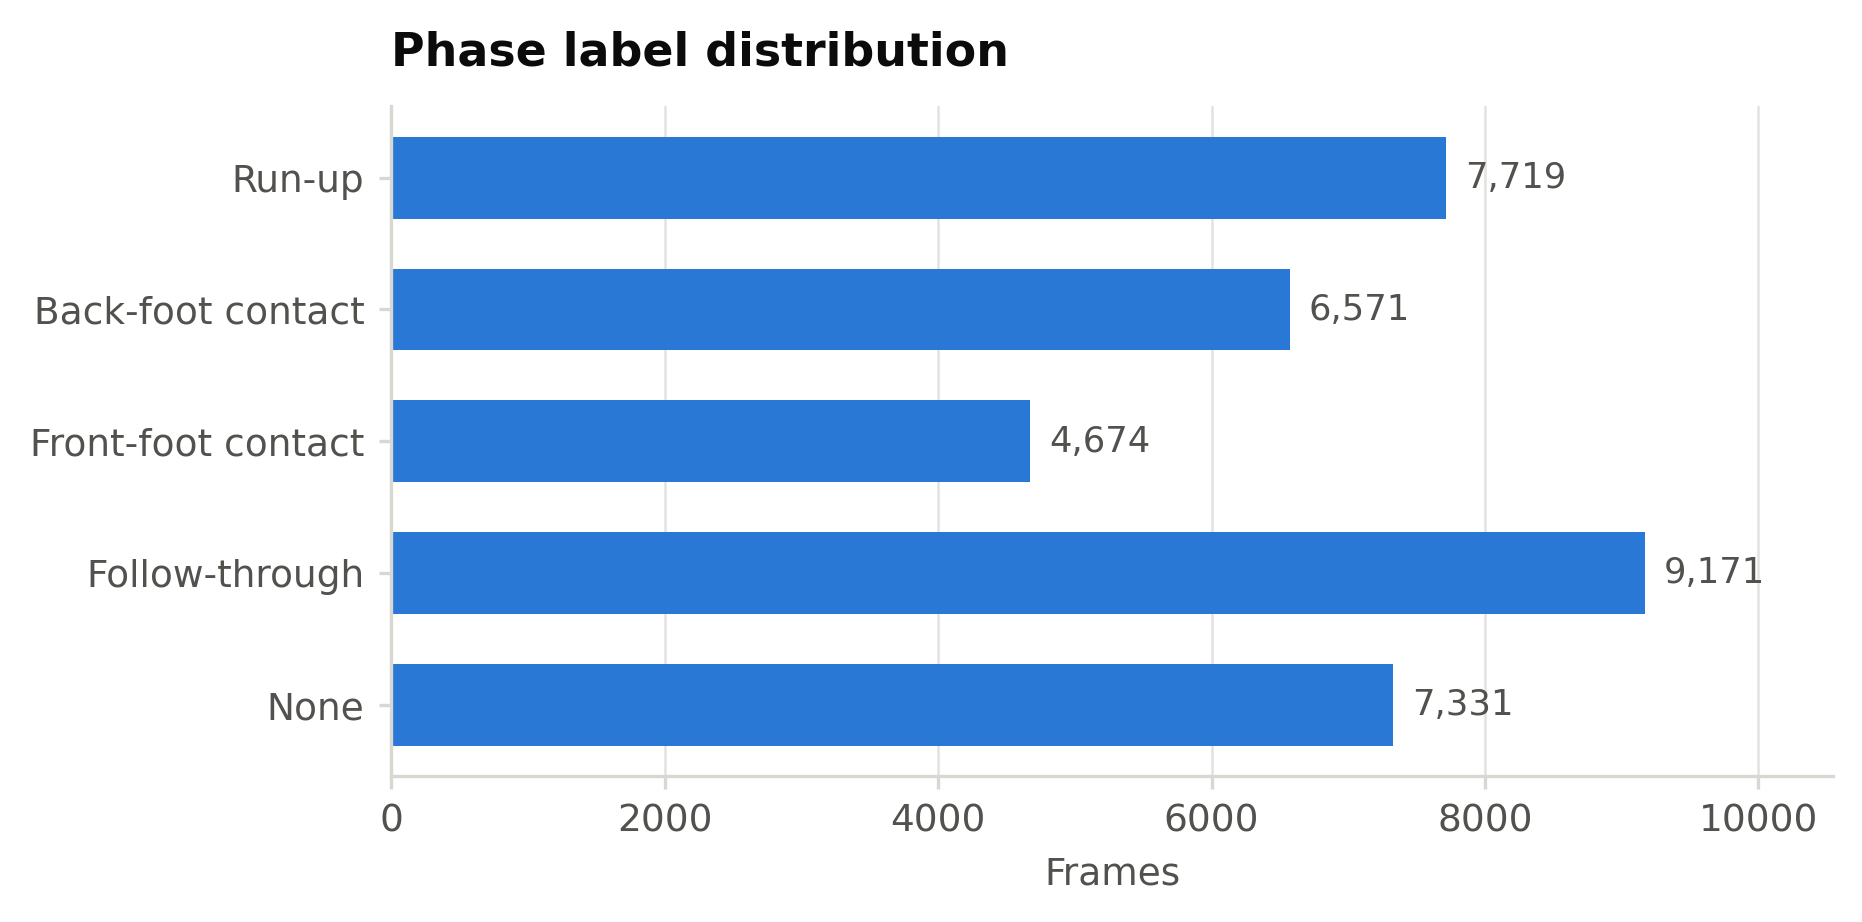
\includegraphics[width=0.78\textwidth]{fig1_class_balance.png}
  \caption{Phase label distribution across 35{,}466 annotated frames. The two
  contact phases are the least frequent and the most important, which is why
  class weighting is applied throughout.}
  \label{fig:balance}
\end{figure}

\section{Methodology}
\label{sec:method}

\subsection{Events versus phases}

An \emph{event} is an instant---a single frame. A \emph{phase} is an
interval. This distinction determines the entire method. Training a classifier
to recognise an event means one positive example per delivery against several
hundred negatives, and the frame immediately before release is visually almost
identical to release itself.

Training on phases is a well-posed problem: each class has thousands of
examples, and the classes are visually distinguishable. We therefore
label every frame with the phase it belongs to, train on that, and read the
events off the boundaries:

\begin{itemize}
  \item BFC $=$ the first frame of the predicted \texttt{bfc\_phase} block
  \item FFC $=$ the first frame of the predicted \texttt{ffc\_phase} block
  \item Release $=$ the last frame of the predicted \texttt{ffc\_phase} block
\end{itemize}

A second benefit follows. Because only the block \emph{edges} are read, the
model may be wrong in the \emph{middle} of a block without affecting the
extracted events. Per-frame accuracy therefore understates event accuracy, and
the two are not interchangeable---a point Section~\ref{sec:disagree} develops
into a result.

\subsection{Pose estimation}

MediaPipe Pose Landmarker (\texttt{heavy}) produces 33 body landmarks per
frame with per-landmark visibility. The \texttt{heavy} variant was chosen
because ankle and wrist positions at ball release are the fastest-moving and
hardest landmarks in the sequence.

\subsection{Normalisation: the substitute for calibration}

Raw landmarks depend on where the bowler stood, how far the phone was, the
image aspect ratio, which way the bowler ran and which arm they bowled with.
Four operations remove all of it.

\paragraph{Aspect correction.} Landmark coordinates are normalised to $[0,1]$
independently on each axis, so on a 16:9 frame equal numeric distances are
unequal real distances. Multiplying $x$ by $W/H$ restores isotropy. Omitting
this step distorts every computed angle; a true $45^\circ$ limb reads as
approximately $68^\circ$.

\paragraph{Direction.} A straight line is fitted to the hip midpoint's
horizontal position over the clip. A positive slope means left-to-right travel;
otherwise $x$ is negated. Direction is recovered from the data, not supplied by
an operator.

\paragraph{Body-relative frame.} With $\mathbf{h}$ the hip midpoint,
$\mathbf{s}$ the shoulder midpoint and $T = \lVert \mathbf{s} - \mathbf{h}
\rVert$ the torso length, every landmark $\mathbf{p}$ becomes
\[
  \mathbf{q} = \frac{\mathbf{p} - \mathbf{h}}{T}.
\]
Translation removes position in frame; division by torso length removes camera
distance and body size. A bowler filmed at 8\,m and one at 15\,m in the same
pose yield identical features. \textbf{This is what replaces camera
calibration.}

\paragraph{Order statistics.} No feature refers to left or right. The
\emph{leading} leg is whichever ankle is further forward; the \emph{high} arm
is whichever wrist is higher. A left-arm bowler's leading leg is their right
and a right-arm bowler's is their left, so defining features by role rather
than by side eliminates handedness entirely---with no flag that can be set
backwards.

Sixteen features result: four joint angles, eight distances in torso units,
and four orientation measures.

\subsection{Window stacking}

A single frame cannot express motion, yet a human identifies front foot contact
by seeing the foot \emph{stop}. Each frame is therefore given the feature
values of its neighbours at offsets $\pm 1 \dots \pm 5$, plus three difference
channels per feature:
\[
  f^{d1}_i = f_i - f_{i-1}, \qquad
  f^{d3}_i = f_i - f_{i-3}, \qquad
  f^{v}_i  = \tfrac{1}{2}\left(f_{i+1} - f_{i-1}\right).
\]
Sixteen features become $16 \times (1 + 10 + 3) = 224$. Windows are built per
clip and clamped at clip boundaries so no frame borrows from another delivery.

We note that this operation is a one-dimensional convolution of width 11 with
hand-set weights. Section~\ref{sec:ablation} measures what the window buys, and
Section~\ref{sec:models} tests whether learning those weights instead helps.

\subsection{Validation protocol}
\label{sec:protocol}

Evaluation uses \textbf{GroupKFold with the bowler as the group}: 24 folds,
each holding out one complete bowler. This is the central methodological
choice. Splitting by frame would place frames 8.3\,ms apart---visually near
identical---in both training and test sets, producing an accuracy figure that
measures memorisation rather than generalisation. Every number reported here
comes from a model that never saw the test bowler.

One bowler was excluded from the classifier entirely. He is not a trained
bowler, and all sixteen of his deliveries were judged illegal. The classifier
therefore trains on 24 bowlers and 27{,}840 frames, and event detection is
evaluated on the other bowlers' 268 deliveries: the 284 usable clips less his 16.

That exclusion is measured rather than asserted. A forest trained on the other
24 bowlers, which is exactly the model his held-out fold would use, still finds
his back foot contact within 3 frames on 12 of his 16 clips, but finds no
front-foot-contact block at all in 15 of the 16. On the one clip where it does,
release is placed 10 frames early, against a mean error of 0.76 frames for
everyone else. His front-foot phase does not resemble anyone else's, so the
exclusion reflects a property of the action, not a convenience.

\subsection{Event extraction}

Per-frame predictions are converted to instants in four steps. Class
probabilities are median-filtered over 9 frames---filtering probabilities
rather than hard labels removes spikes without dragging block edges. Contiguous
blocks are identified. The \texttt{bfc\_phase} and \texttt{ffc\_phase} blocks
maximising combined confidence are selected \emph{subject to the constraint
that the BFC block begins first}, which is true of every bowling action ever
performed and rescues clips where a spurious fragment appears after release.
Events are then read off the block edges.

\textbf{A clip in which no block is found counts as a failure}, not as a
missing value. Rates reported below are shares of all 268 deliveries, so a
model that declines the hard cases is not rewarded for it.

\subsection{From measurements to a usable tool}
\label{sec:tool}

The pipeline is packaged as a website, Delivery Stride
(\url{https://tarak-ram-1908.github.io/Fast-Bowling/}). A bowler uploads up
to six side-on clips of at most twelve seconds each and receives the
measurements for every delivery and their average, each compared with the
elite reference. The whole analysis runs in the visitor's web browser: the
same MediaPipe pose model, a JavaScript port of the features, random forest,
event extraction and measurements, so the video never leaves the device and
no server is needed.

A single clip is a much weaker measurement than the cohort, mostly because
back foot contact is right only 59\% of the time, so the report guards each
delivery. The three event frames are shown with the detected skeleton and can
be stepped forwards or backwards and re-measured. Every value is checked
against our own 262 deliveries: past three cohort standard deviations it is
reported as a probable detection error rather than a finding. Each
measurement carries a confidence level inherited from the event frames it
depends on, and every value more than one standard deviation from the elite
mean is drawn on the frame it was measured at, beside where the elite average
would put the same segments. Explanations quote the published association
across bowlers and never prescribe a change.

Fed the same pose landmarks, the browser port reproduces the Python pipeline
exactly on six clips from five bowlers: every event, measurement, confidence
level and warning. Run end to end in the browser on three clips, all nine
detected events matched the Python version frame for frame.

\section{Experimental Results}
\label{sec:results}

\subsection{Event detection}

\begin{table}[htbp]
  \centering
  \caption{Event detection accuracy (forest), leave-one-bowler-out. Rates are out of all 268 deliveries; 'Detected' is how many yielded a phase block at all. 'Error' is the mean absolute timing error, in frames and in milliseconds, over the deliveries detected.}
  \label{tab:events}
  \small
  \begin{tabular}{lrrrrrr}
    \toprule
    Event & Detected & Error (fr) & Error (ms) & Within 1 & Within 3 & Within 5 \\
    \midrule
    Ball release & 268/268 & 0.76 & 6.3 & 86.6\% & 98.5\% & 99.6\% \\
    Front-foot contact & 268/268 & 1.53 & 12.7 & 59.3\% & 91.8\% & 98.9\% \\
    Back-foot contact & 267/268 & 3.54 & 29.5 & 25.7\% & 59.0\% & 78.7\% \\
    \bottomrule
  \end{tabular}
\end{table}


\begin{figure}[H]
  \centering
  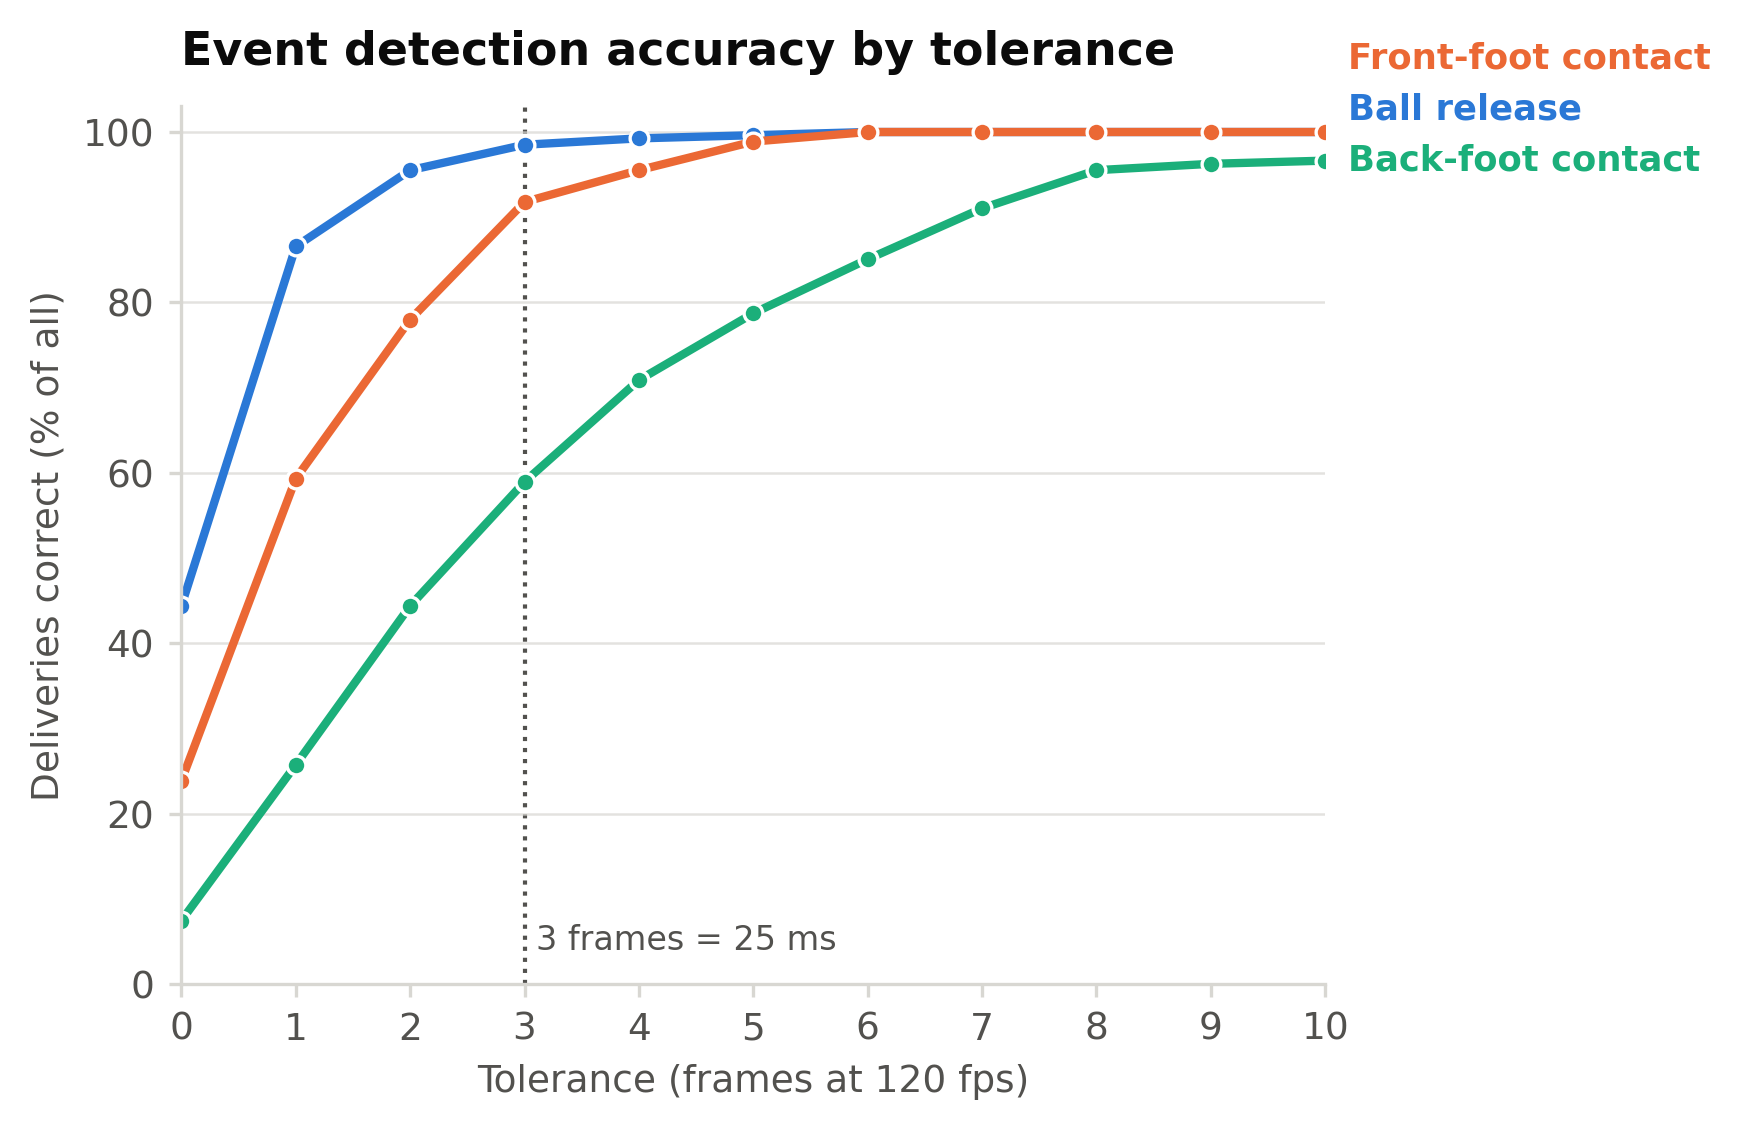
\includegraphics[width=0.82\textwidth]{fig2_tolerance.png}
  \caption{Event detection accuracy as a function of tolerance, random forest,
  leave-one-bowler-out, as a share of all 268 deliveries. The three curves
  separate in the order release, front foot contact, back foot
  contact---which is the order of how sharply each event is defined in the
  video.}
  \label{fig:tolerance}
\end{figure}

Ball release is located within 3 frames on 98.5\% of deliveries with a mean
absolute error of 0.76 frames (6.3\,ms). Front foot contact reaches 91.8\%.
Back foot contact reaches 59.0\%, with a mean error of 3.54 frames (29.5\,ms).
Both contacts fall within 3 frames on 53.0\% of deliveries (142 of 268).

Two observations about the weakest result. First, the ordering is physical:
the ball separates visibly from the hand, the front foot brakes sharply, and
the back foot \emph{rolls} through rather than arriving. Second, this ordering
matches an independent finding in gait analysis, where published limits of
agreement for trained human annotators are 24\,ms for heel strike and 16\,ms
for toe-off, but rise to 72\,ms for heel-off and 80\,ms for flat
foot~\cite{gait2022}---the events where the foot rolls. Our mean release error
of 6.3\,ms is smaller than the published disagreement between humans on any of
those events.

\subsection{Does window stacking help?}
\label{sec:ablation}

Window stacking is claimed as a contribution, so it is tested directly. The
pipeline was run end to end twice on identical folds and identical bowlers,
differing only in whether the $\pm5$ window and its difference channels were
present. Both runs count a clip with no phase block as a failure, and all
rates are shares of the same 268 deliveries.

\begin{table}[htbp]
  \centering
  \caption{Window stacking ablation. Random forest, 24 bowlers, 27{,}840
  frames, leave-one-bowler-out, identical folds. The 16 base features alone
  against the same features stacked across $\pm5$ frames with first
  differences (224 columns).}
  \label{tab:ablation}
  \small
  \begin{tabular}{lrr}
    \toprule
     & 16 features & 224 stacked \\
    \midrule
    Per-frame accuracy & 80.0\% & \textbf{85.2\%} \\
    Ball release within 3 frames & 94.4\% & \textbf{98.5\%} \\
    Front foot contact within 3 frames & 88.1\% & \textbf{91.8\%} \\
    Back foot contact within 3 frames & 51.1\% & \textbf{59.0\%} \\
    Both contacts within 3 frames & 42.5\% & \textbf{53.0\%} \\
    \midrule
    Mean release error & 1.00 fr (8.4\,ms) & \textbf{0.76 fr (6.3\,ms)} \\
    Fragmented phase blocks & 25 & \textbf{4} \\
    Clips with no block found & 2 & \textbf{1} \\
    \bottomrule
  \end{tabular}
\end{table}

Every measure improves. The two that matter most are at the bottom: fragmented
blocks fall from 25 to 4, and the share of deliveries where \emph{both} contacts
land within 3 frames rises by more than ten percentage points. Fragmentation is
the failure mode that breaks event extraction outright---a phase predicted as
two blocks with a gap has no single edge to read---so reducing it is worth more
than the per-frame accuracy gain suggests.

The back foot contact gain (51.1\% to 59.0\%) is the largest of the three
events, which is consistent with the account in Section~\ref{sec:disagree}: the
diffuse event benefits most from temporal context, and $\pm5$ frames is the
smallest amount of context that helps it.

\subsection{Model comparison}
\label{sec:models}

Seven models were trained on identical folds. Each answers a question rather
than filling a row: logistic regression is the linear baseline; the random
forest is the incumbent; extremely randomised trees test whether the forest
overfits through its split thresholds; gradient boosting is the strongest
classical competitor on tabular data; the MLP tests whether a dense network
alone helps; the TCN learns the convolution that window stacking performs by
hand; and the bidirectional LSTM can learn temporal ordering that is otherwise
imposed afterwards.

\begin{table}[htbp]
  \centering
  \caption{Per-frame phase classification, leave-one-bowler-out.}
  \label{tab:models_perframe}
  \begin{tabular}{lrr}
    \toprule
    Model & Accuracy & Macro F1 \\
    \midrule
    bilstm & 0.915 & 0.909 \\
    extratrees & 0.847 & 0.827 \\
    forest & 0.852 & 0.831 \\
    hgb & 0.863 & 0.844 \\
    logreg & 0.816 & 0.806 \\
    mlp & 0.843 & 0.822 \\
    tcn & 0.833 & 0.820 \\
    \bottomrule
  \end{tabular}
\end{table}


\begin{figure}[H]
  \centering
  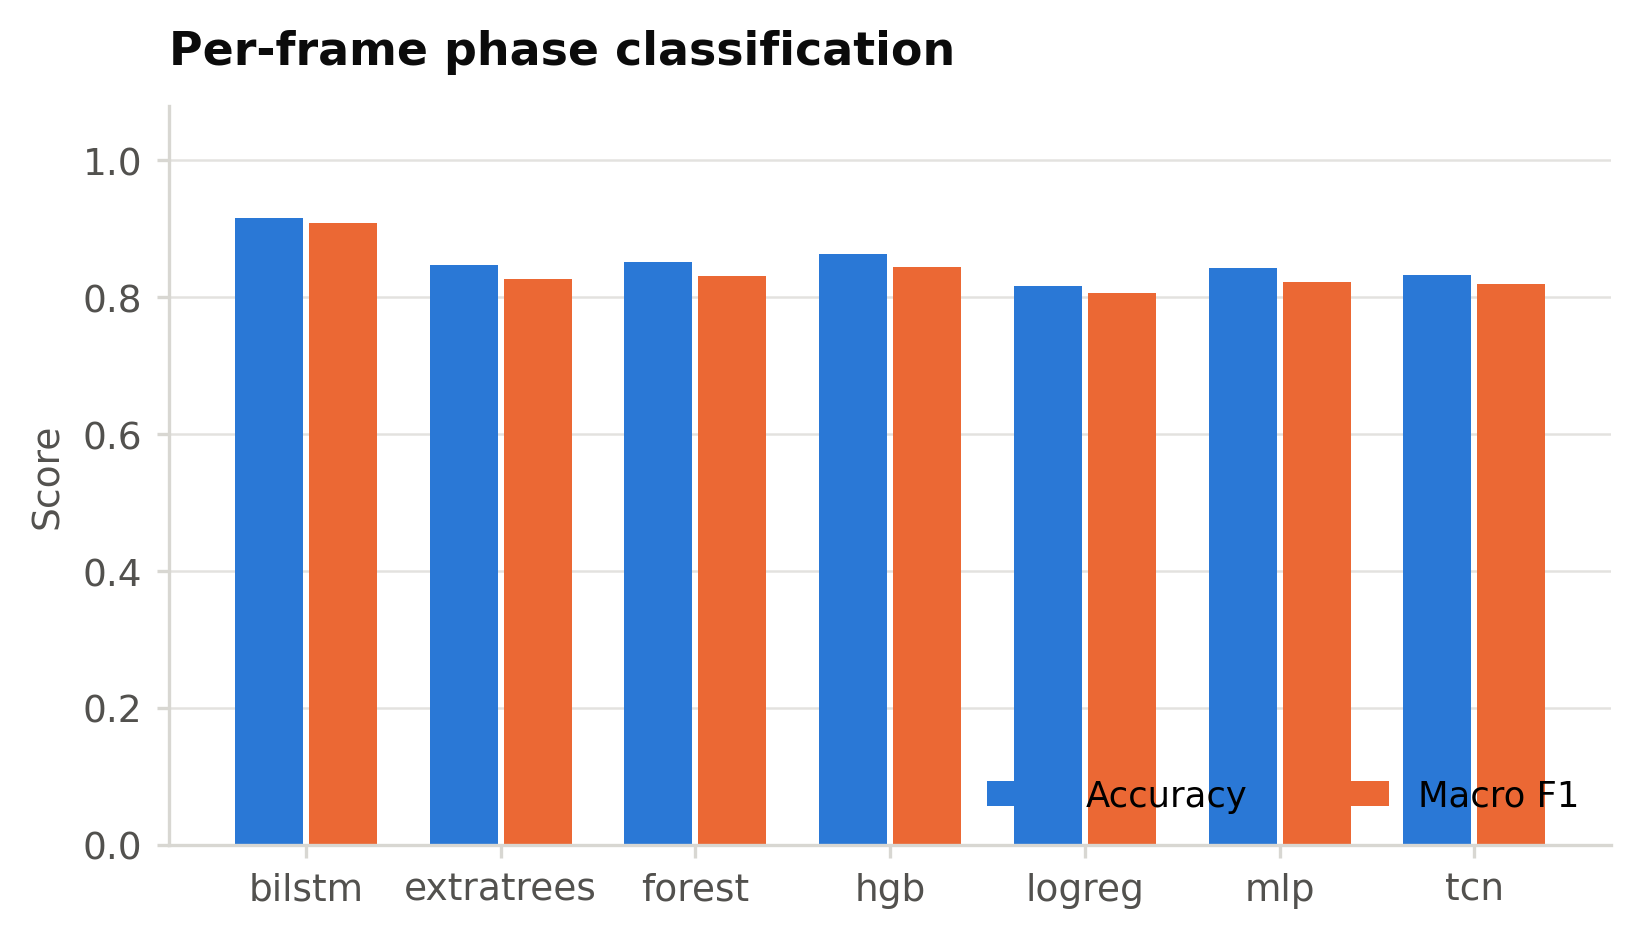
\includegraphics[width=0.82\textwidth]{fig3_models_perframe.png}
  \caption{Per-frame accuracy and macro F1, leave-one-bowler-out. Exact
  values are in Table~\ref{tab:models_perframe}.}
  \label{fig:perframe}
\end{figure}

\subsection{Per-frame accuracy and event accuracy disagree}
\label{sec:disagree}

\begin{table}[htbp]
  \centering
  \caption{Event detection within 3 frames, by model, as a share of all deliveries (clips where no block was found count as failures).}
  \label{tab:models_events}
  \begin{tabular}{lrrrrrrr}
    \toprule
    Event & bilstm & extratrees & forest & hgb & logreg & mlp & tcn \\
    \midrule
    Ball release & 97.4\% & 98.5\% & 98.5\% & 98.5\% & 88.1\% & 96.3\% & 88.4\% \\
    Front-foot contact & 72.8\% & 84.7\% & 91.8\% & 91.0\% & 80.6\% & 83.2\% & 82.1\% \\
    Back-foot contact & 79.9\% & 58.2\% & 59.0\% & 59.0\% & 53.4\% & 59.0\% & 49.6\% \\
    \bottomrule
  \end{tabular}
\end{table}


\begin{figure}[H]
  \centering
  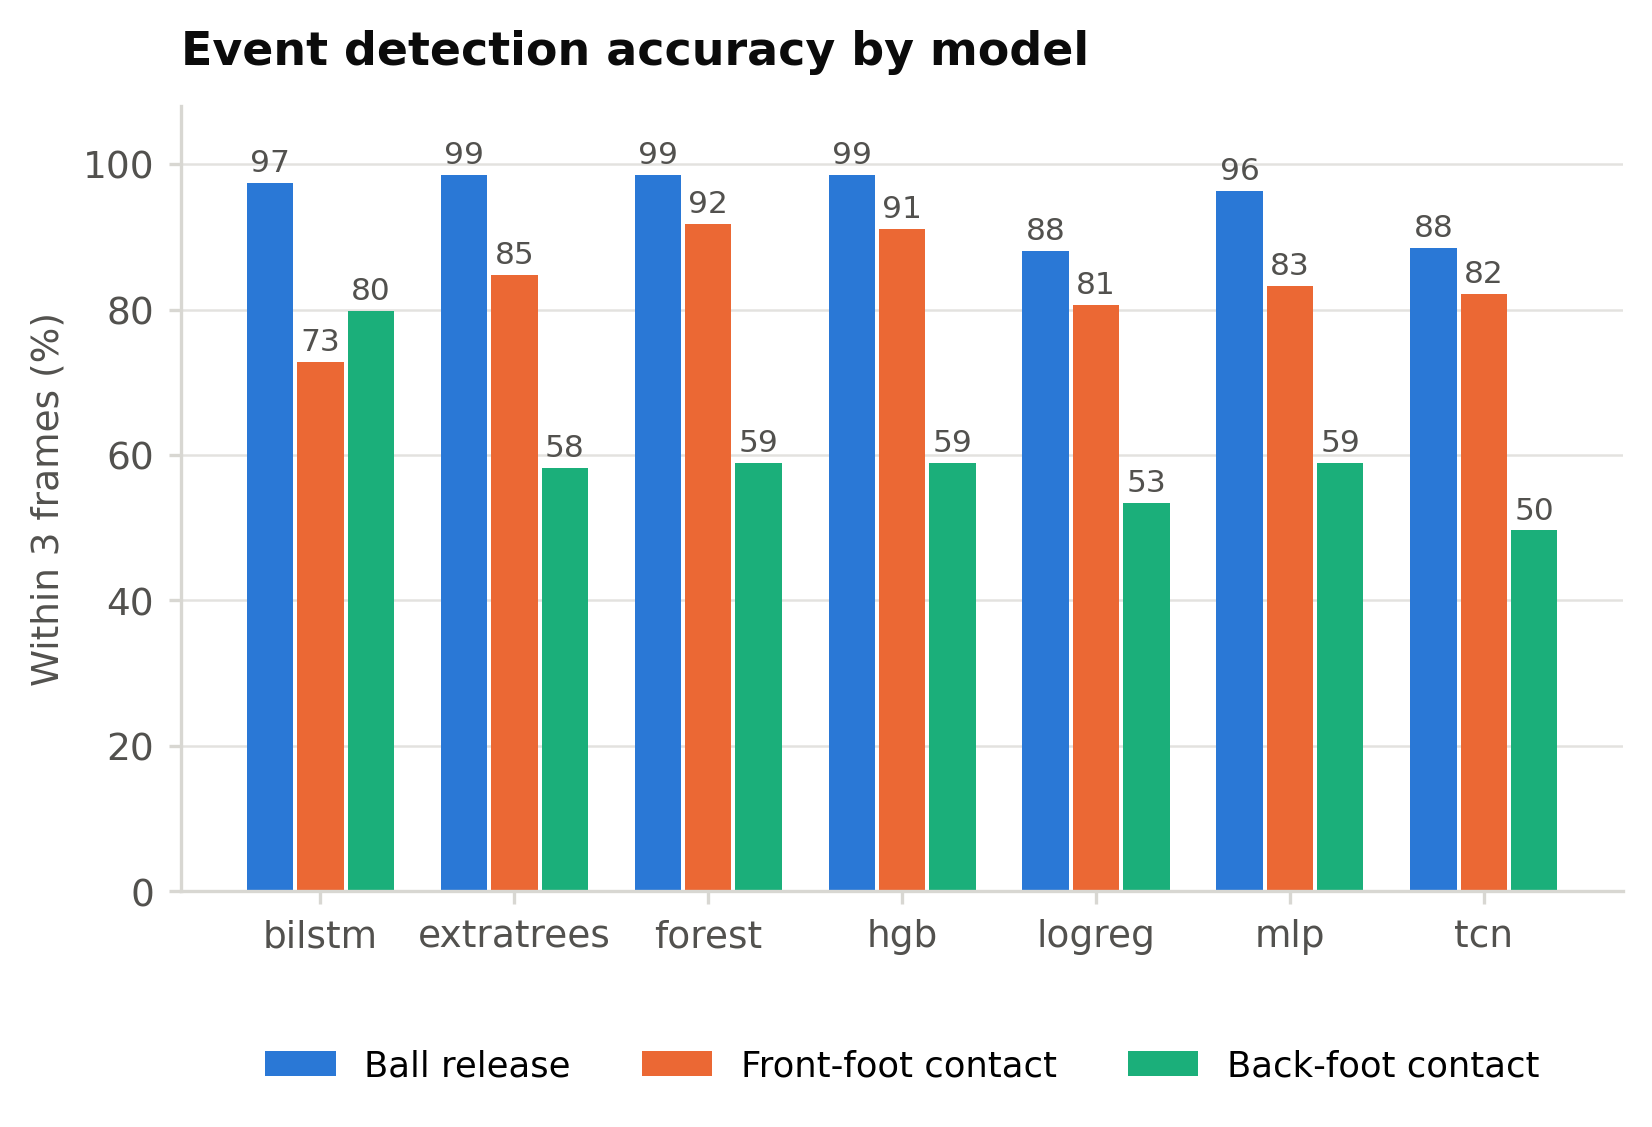
\includegraphics[width=0.82\textwidth]{fig4_models_events.png}
  \caption{Event detection within 3 frames, by model, as a share of all 268
  deliveries. Compare the ordering here with Figure~\ref{fig:perframe}.}
  \label{fig:modelevents}
\end{figure}

The two rankings do not agree. The bidirectional LSTM leads per-frame accuracy
by more than five points (0.915 against 0.863 for the next best) yet is
\textbf{the worst of all seven models at front foot contact}, at 72.8\% against
the forest's 91.8\%---while simultaneously being by far the best at back foot
contact, at 79.9\% against 59.0\%.

Both halves of that trade have the same explanation. Back foot contact is
diffuse: the foot rolls, no single frame is distinguished, and the instant must
be inferred from the rhythm of the whole stride, which is exactly what
long-range bidirectional context supplies. Front foot contact is sharp: the
braking signature is local, a window of $\pm 5$ frames already captures it, and
smoothing over a long context blurs the boundary.

We further caution that the LSTM's per-frame advantage is partly an artefact.
Its largest per-class gain is on the \texttt{none} class (F1 0.892 against
0.623 for the forest), which denotes frames outside the delivery. Those are
determined largely by where each clip was trimmed, and a model reading the
whole sequence can learn clip position rather than biomechanics. This cannot
affect the event results, which read only the two contact-phase blocks, but it
does mean the 0.915 figure should not be quoted as a capability.

Compute cost differs by more than an order of magnitude and is worth recording:
extremely randomised trees reached 0.847 in 236\,s where the random forest
reached 0.852 in 5{,}052\,s, and gradient boosting beat the forest outright in
a sixth of its time.

\begin{figure}[H]
  \centering
  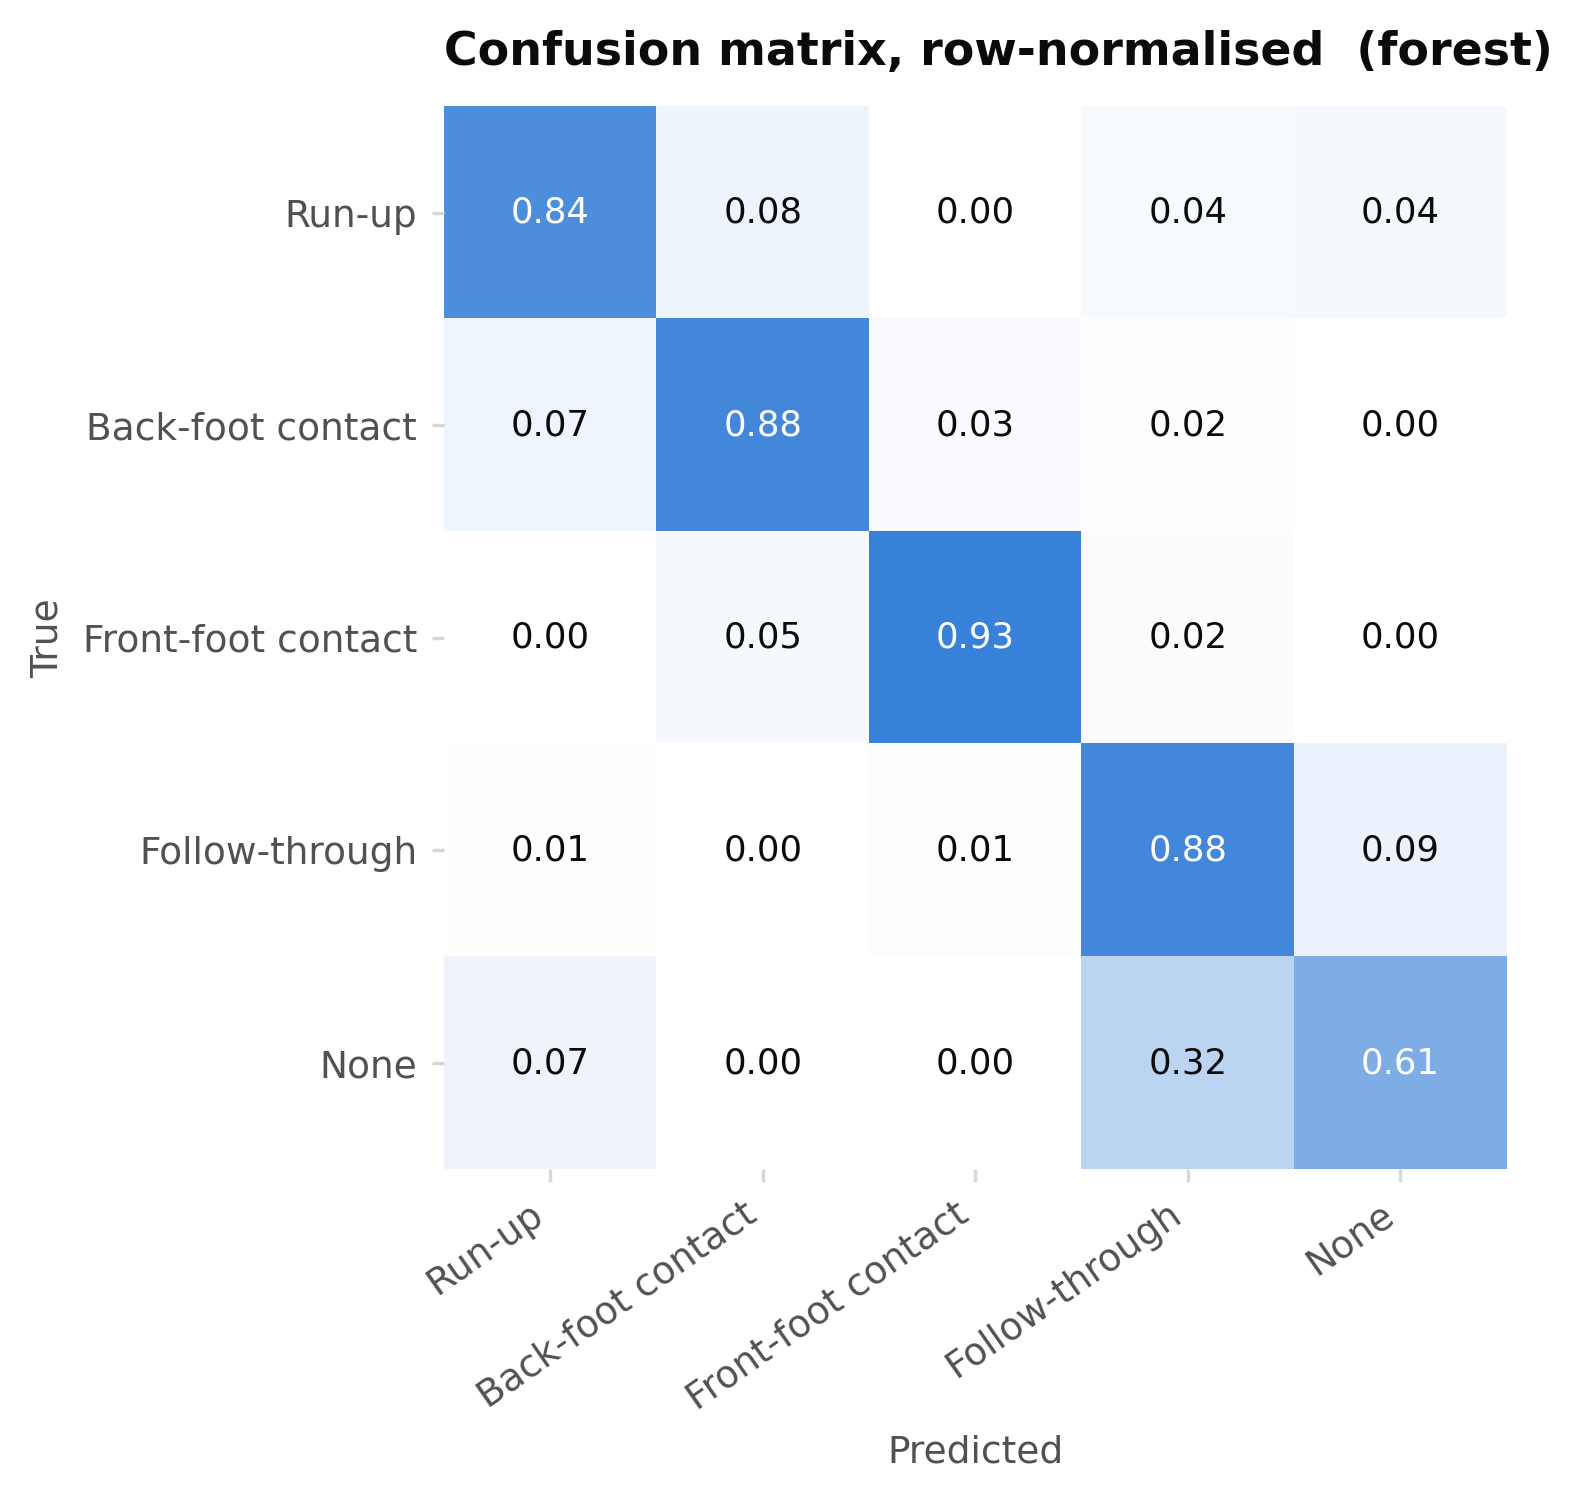
\includegraphics[width=0.70\textwidth]{fig5_confusion.png}
  \caption{Row-normalised confusion matrix for the random forest, the model
  reported throughout. Confusions concentrate between adjacent phases, which
  is the benign failure mode: an error in the middle of a block does not move
  its edge.}
  \label{fig:confusion}
\end{figure}

\begin{figure}[H]
  \centering
  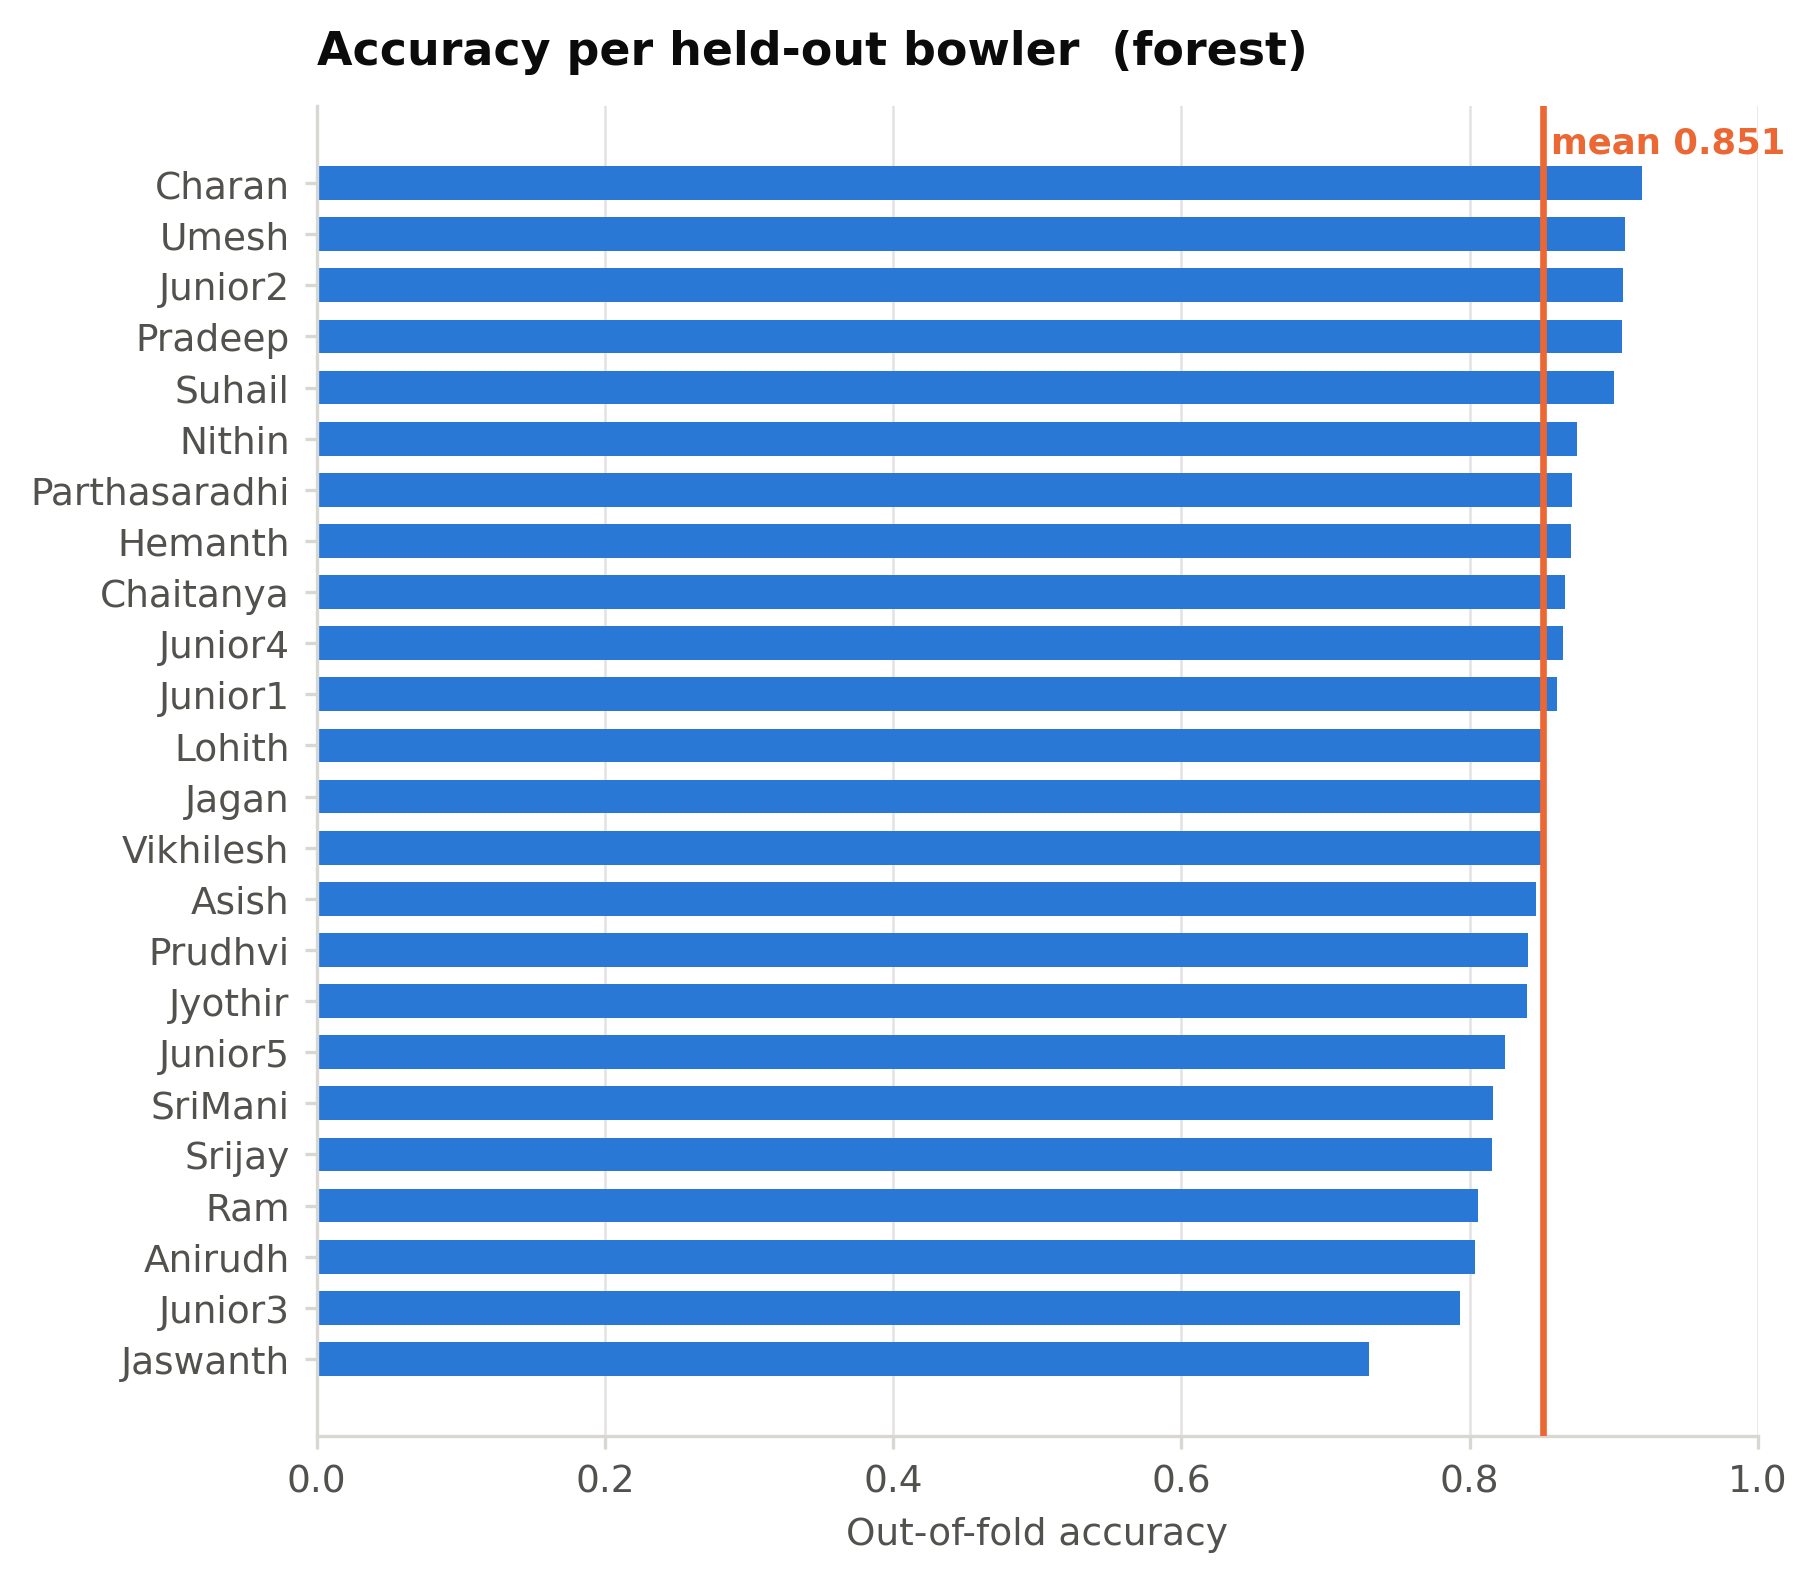
\includegraphics[width=0.82\textwidth]{fig7_per_bowler.png}
  \caption{Random forest accuracy on each held-out bowler. The spread matters
  more than the mean for a system intended to work on someone it has never
  seen.}
  \label{fig:perbowler}
\end{figure}

\subsection{Kinematic measurement}

Eight variables were computed at the detected instants on 262 legal deliveries
from 23 bowlers, and compared with Worthington's elite
values~\cite{worthington2010}. Lengths are reported as a percentage of standing
height, obtained from torso-relative measurements using the anthropometric
constant $0.288$ of Winter~\cite{winter1990}: the shoulder joint sits at
$0.818H$ and the hip at $0.530H$, so the trunk spans $0.288H$. Standing heights
were measured for 24 of the 25 bowlers, but they are not used in any figure
reported here: every length is converted with the trunk ratio alone.

Each variable follows Worthington's definition as closely as a single sagittal
view allows. Stride length is the distance between the two ankle joint centres
at the instant of front foot contact, as he defines it; only the along-pitch
component is visible, and the across-pitch part of a typical stride adds about
2\,cm. Knee angle is signed in the sagittal plane, so a knee past straight
reads above $180^\circ$ as in his data, whose range at release reaches
$186.2^\circ$; an unsigned interior angle would fold such a knee back to read
as flexed. Plant angle (hip to ankle against the downward vertical),
foot-strike indicator (ankle to toe against the horizontal) and lean-back
(back ankle to shoulder midpoint against the vertical) are his projected
two-dimensional angles directly. One variable is measured but \emph{not}
compared: Worthington takes knee flexion from \emph{front foot flat}, the
instant the whole foot is down, which this system does not detect. Measured
from front foot contact instead, flexion reads several degrees higher---a
heuristic estimate of foot flat puts the difference at a median of $5.6^\circ$
across our deliveries---so a comparison would overstate it.

\begin{table}[htbp]
  \centering
  \caption{Measured kinematics against Worthington (2010) elite reference values. Ours and Elite are mean $\pm$ sd. $z$ is the shift of our mean in elite standard deviations; the final column is the share of our individual deliveries falling inside the elite one-sd band.}
  \label{tab:measurements}
  \footnotesize
  \begin{tabular}{lrrrrr}
    \toprule
    Measurement & n & Ours & Elite & $z$ & In $\pm$1\,sd \\
    \midrule
    Front knee at FFC & 262 & 167.8 $\pm$ 8.4 & 164.1 $\pm$ 6.1 & +0.60 & 47\% \\
    Front knee at release & 262 & 143.4 $\pm$ 17.6 & 167.3 $\pm$ 18.8 & -1.27 & 33\% \\
    Knee flexion & 262 & 27.5 $\pm$ 15.0 & 17.5 $\pm$ 11.2 & +0.89 & 38\% \\
    Knee extension & 262 & 3.1 $\pm$ 4.5 & 11.9 $\pm$ 7.4 & -1.19 & 24\% \\
    Plant angle & 262 & 36.6 $\pm$ 4.6 & 36.3 $\pm$ 3.9 & +0.07 & 61\% \\
    Foot strike & 262 & 7.1 $\pm$ 13.7 & -8.2 $\pm$ 13.2 & +1.16 & 37\% \\
    Trunk lean at BFC & 262 & 3.4 $\pm$ 5.7 & 9.0 $\pm$ 5.2 & -1.09 & 47\% \\
    Stride (\% height) & 262 & 67.3 $\pm$ 8.8 & 78.5 $\pm$ 7.2 & -1.56 & 32\% \\
    Release height (\% height) & 262 & 108.3 $\pm$ 10.2 & 112.8 $\pm$ 4.1 & -1.09 & 23\% \\
    \bottomrule
  \end{tabular}
\end{table}


Trunk lean at back foot contact has $n = 261$ rather than 262 because one
legal delivery yielded no back-foot phase block (the 267 of 268 in
Table~\ref{tab:events}), so there is no frame to measure it at.

\begin{figure}[H]
  \centering
  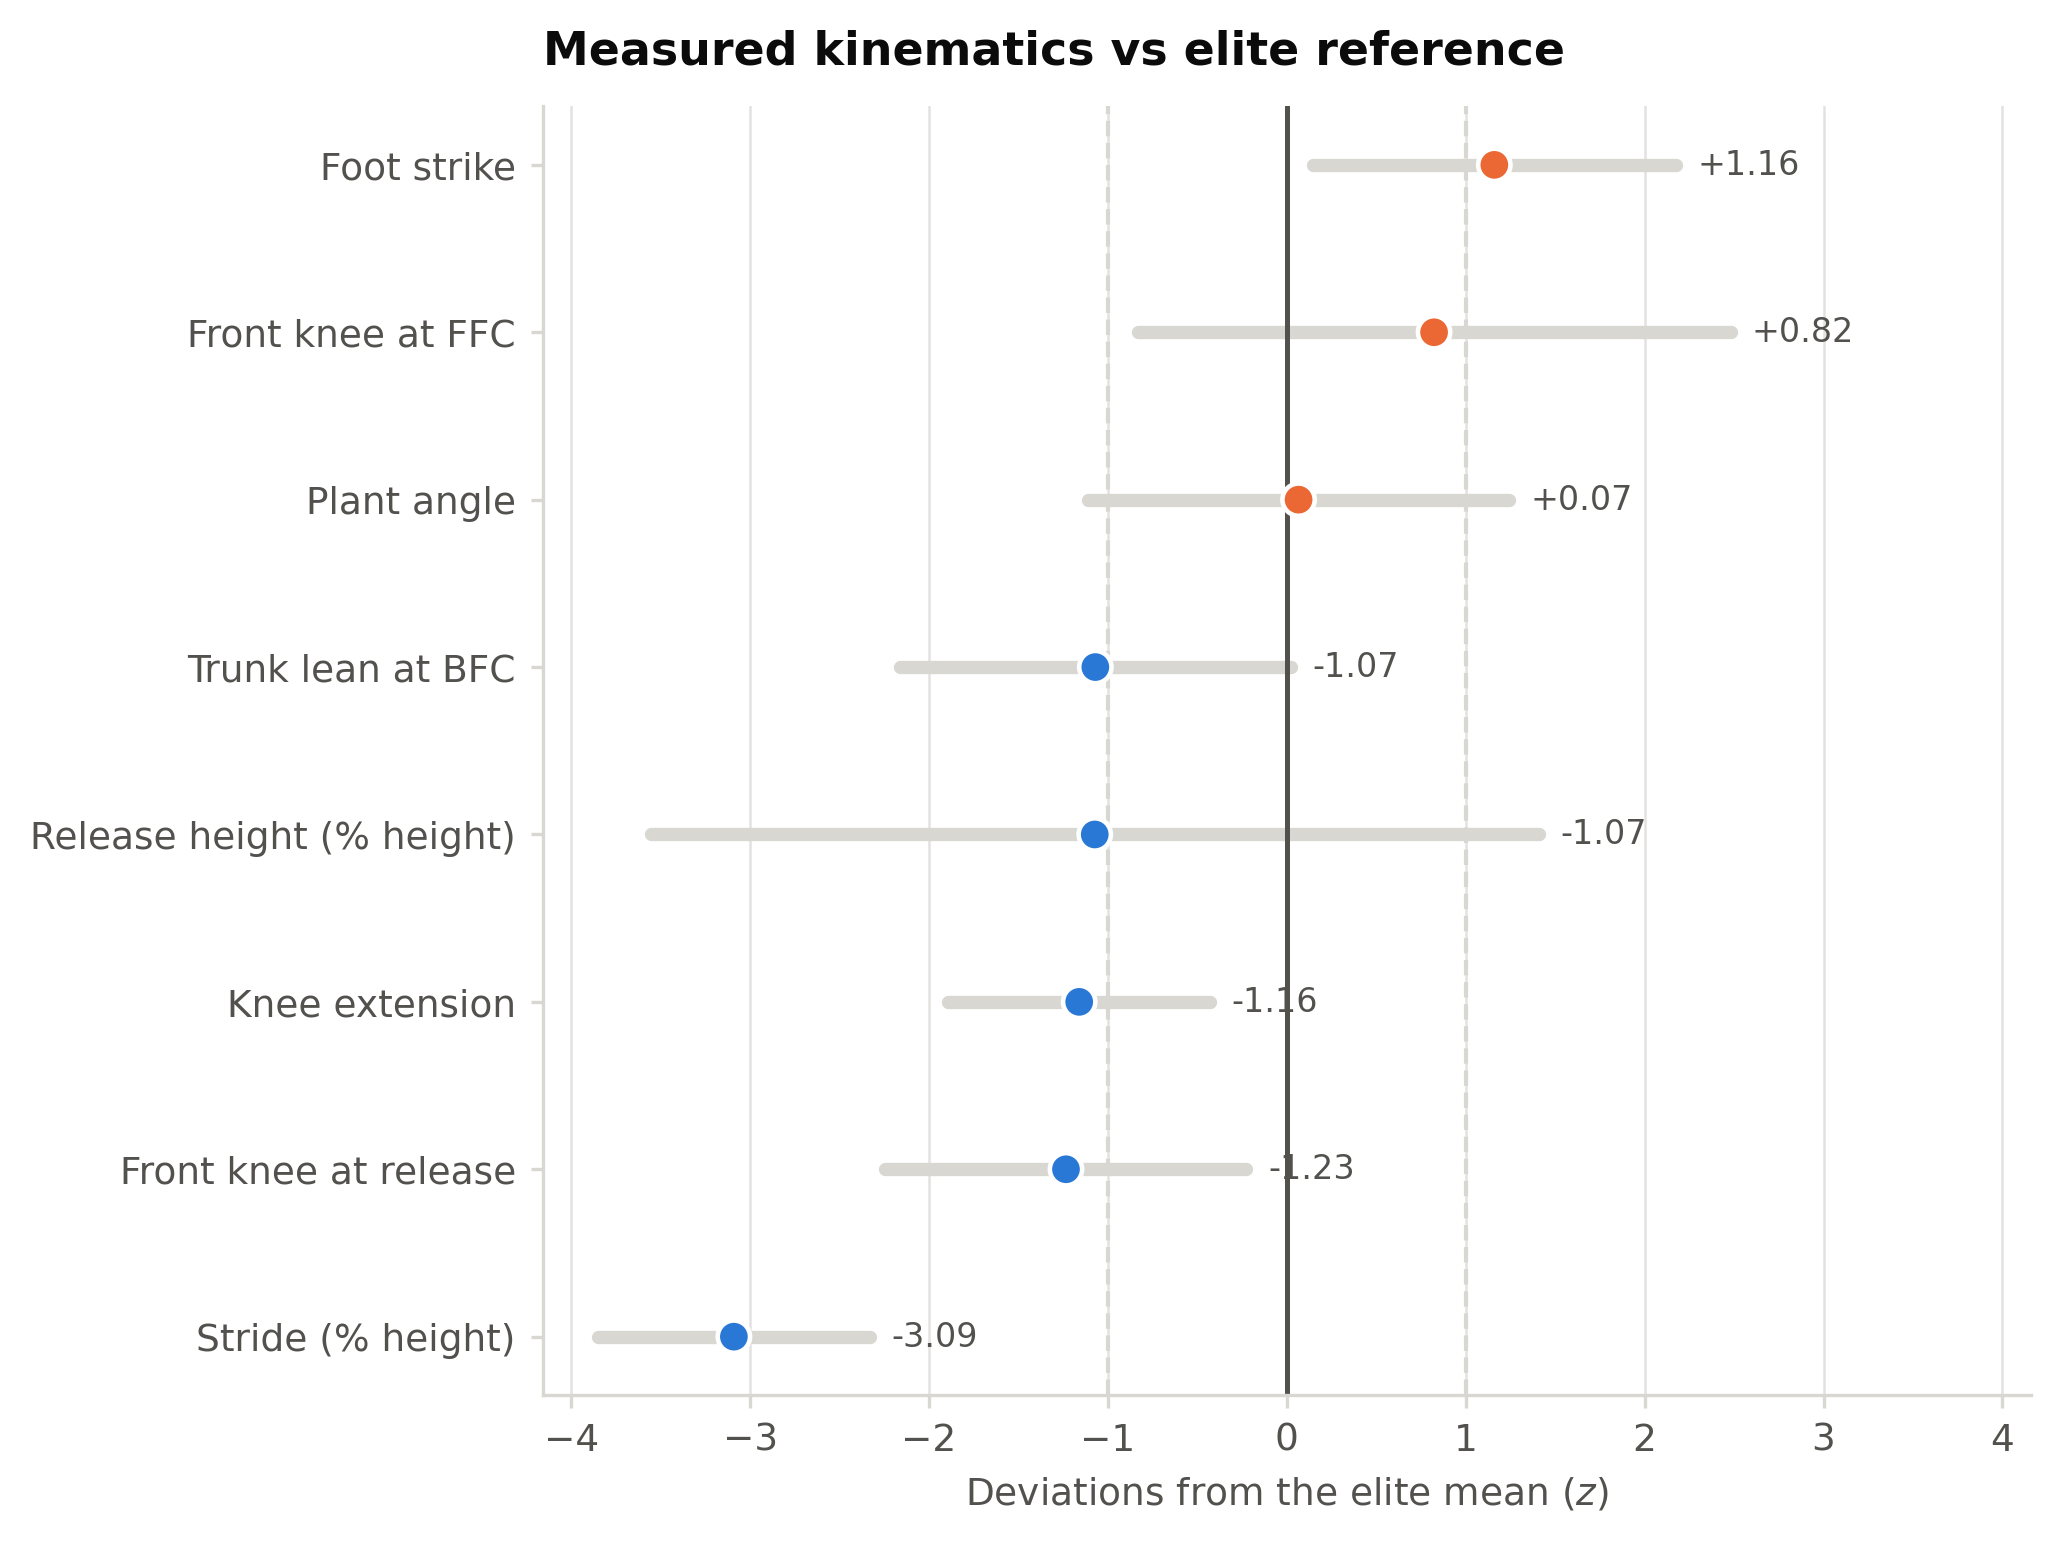
\includegraphics[width=0.82\textwidth]{fig6_measurements.png}
  \caption{Measured kinematics as deviations from the elite mean. The dot is
  our mean; the bar is our own spread (one standard deviation of our
  deliveries, in elite standard deviations). Plant angle sits at $+0.07$,
  which is reassuring: a broken measurement chain would not readily produce
  agreement on one variable and a coherent pattern across the rest. How
  precisely it agrees is limited by timing error
  (Section~\ref{sec:sensitivity}).}
  \label{fig:measurements}
\end{figure}

The table reports our own standard deviation beside the elite one, and the
final column gives the share of our \emph{individual} deliveries falling inside
the elite one-standard-deviation band. Both matter: a shifted mean alone cannot
distinguish a whole group that differs from a handful of outliers dragging an
otherwise typical cohort.

These are not eight independent findings. Read together they describe one
mechanism. Stride is the largest difference in the study: 3.09 standard
deviations shorter than elite, with not one of our 262 deliveries inside the
elite one-standard-deviation band. A short stride leaves the front leg less
braced, so the knee extends less after landing ($-1.16$) and remains more
flexed at release ($-1.23$). Release height is also lower on average ($-1.07$),
though Section~\ref{sec:universal} shows this particular variable varies too
widely between bowlers to be treated as a group property. Reduced backward
trunk lean at back foot contact ($-1.07$) is the same pattern one step earlier.
\textbf{The front leg collapses rather than bracing}. That is consistent with
club bowlers bracing less than professionals, but Section~\ref{sec:technique}
explains why a measurement that compresses knee extension cannot yet be ruled
out.

Foot strike angle ($+1.16$) does not belong to that pattern and is the one
result we cannot currently explain. Footwear is a plausible confounder: the 23
measured bowlers comprised 13 in shoes, 6 in sandals and 4 barefoot, with none
in spikes.

\subsection{What event timing error costs each measurement}
\label{sec:sensitivity}

Every delivery was measured twice: at the frames the classifier predicted, and
at the frames marked by hand. The difference between the two is what the
event timing error, including the 59\% back foot contact rate, actually costs
each measurement. Table~\ref{tab:sensitivity} sets it beside the gap from the
elite mean that the measurement is used to report.

\begin{table}[htbp]
  \centering
  \caption{Mean absolute change in each measurement when it is taken at the
  predicted instead of the hand-marked frames, against our mean's distance
  from the elite mean. 262 legal deliveries (261 for trunk lean).}
  \label{tab:sensitivity}
  \small
  \begin{tabular}{lrr}
    \toprule
    Measurement & Timing cost & Gap from elite \\
    \midrule
    Stride (\% height) & 1.4 & $-22.3$ \\
    Front knee at release & 2.0$^\circ$ & $-23.2^\circ$ \\
    Knee extension & 0.9$^\circ$ & $-8.6^\circ$ \\
    Trunk lean at BFC & 2.8$^\circ$ & $-5.6^\circ$ \\
    Front knee at FFC & 3.3$^\circ$ & $+5.0^\circ$ \\
    Release height (\% height) & 1.4 & $-4.4$ \\
    Foot strike & 7.4$^\circ$ & $+15.3^\circ$ \\
    Plant angle & 1.9$^\circ$ & $+0.3^\circ$ \\
    \bottomrule
  \end{tabular}
\end{table}

The main findings survive it comfortably. Stride, front knee angle at release
and knee extension differ from elite by roughly ten times what timing error can
move them, so the short-stride, collapsing-leg pattern is not an artefact of
missed events. Two rows cut the other way. Plant angle's $0.3^\circ$ agreement
lies inside its own $1.9^\circ$ timing noise, so it shows agreement but cannot
show how close. Foot strike's unexplained $+15.3^\circ$ is only about twice its
$7.4^\circ$ sensitivity, which makes it the least secure difference in the
table.

\subsection{Is the pattern universal?}
\label{sec:universal}

A group mean can be produced either by a cohort that differs uniformly or by a
few extreme individuals. Figure~\ref{fig:perbowlerz} separates the two by
showing every bowler's mean deviation on every variable.

\begin{figure}[H]
  \centering
  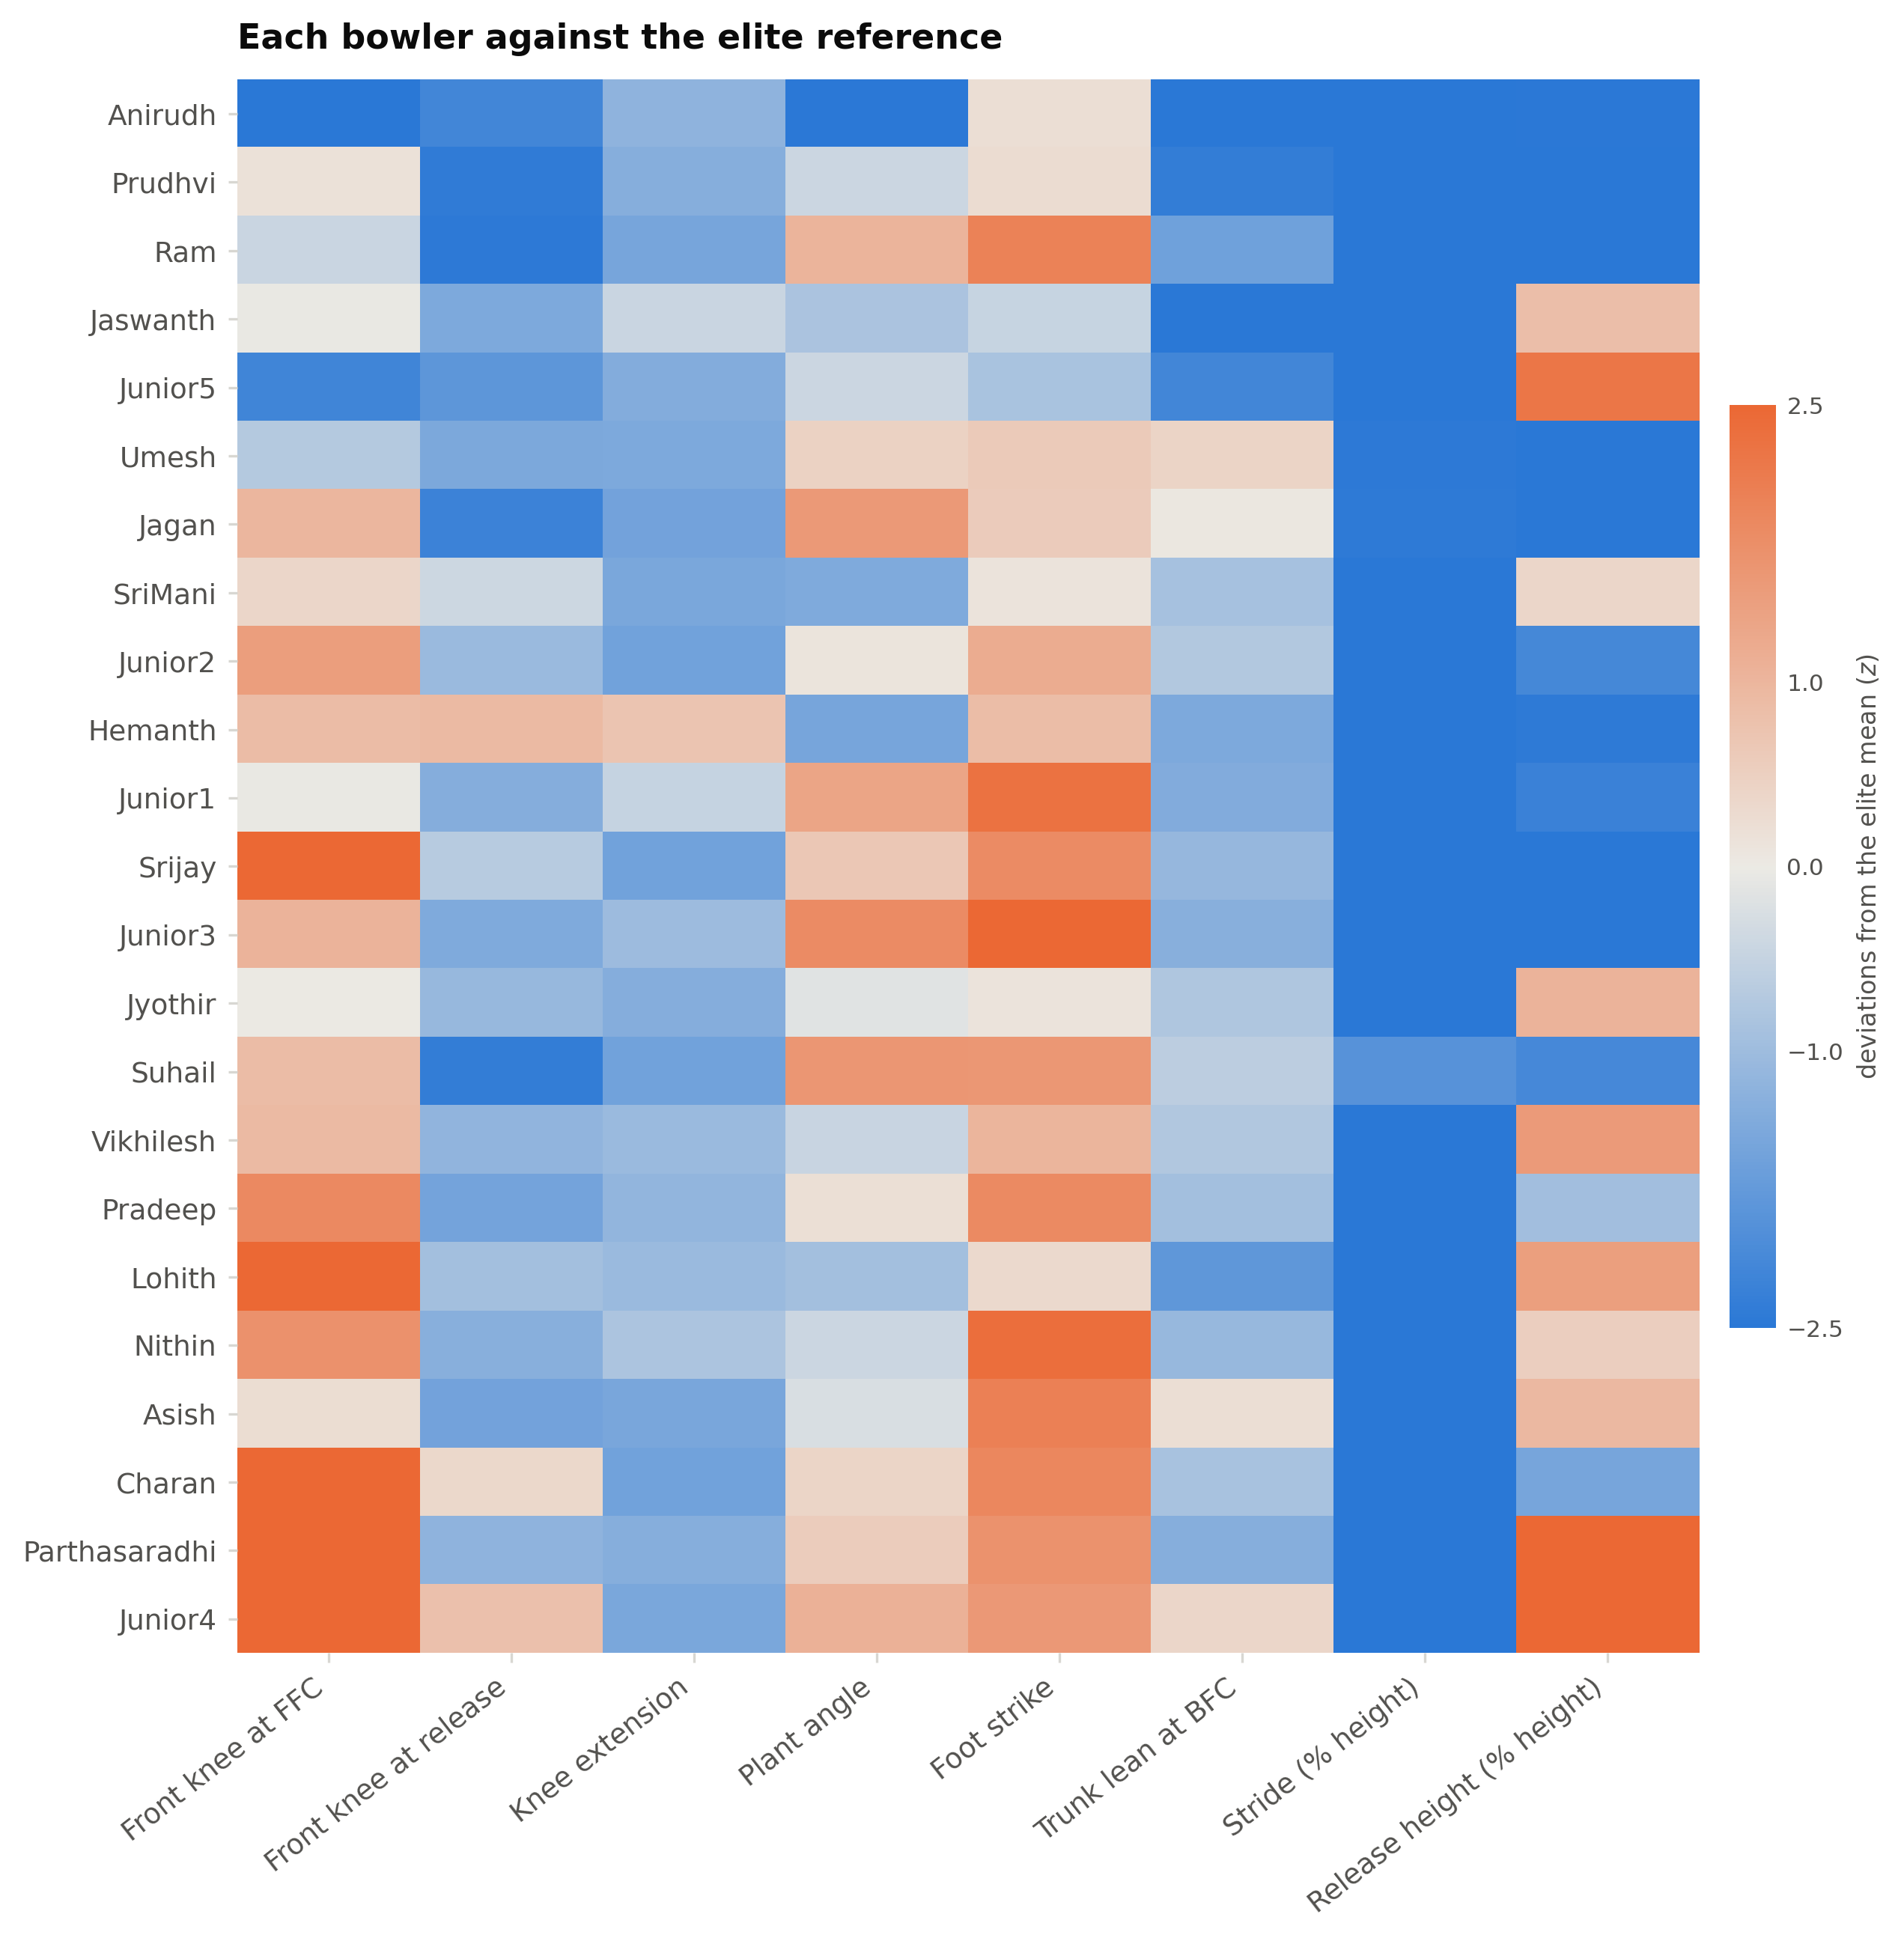
\includegraphics[width=0.95\textwidth]{fig9_per_bowler_z.png}
  \caption{Each bowler against the elite reference, in elite standard
  deviations, sorted by overall deviation. A column of uniform colour means
  the whole cohort differs on that variable; a column with a few saturated
  cells against a pale background means a small number of bowlers carry the
  group mean.}
  \label{fig:perbowlerz}
\end{figure}

\begin{table}[htbp]
  \centering
  \caption{Each bowler's mean deviation from the elite reference, in elite standard deviations, sorted by overall deviation. Columns: Knee$_\text{FFC}$ = Front knee at FFC; Knee$_\text{rel}$ = Front knee at release; Flex = Knee flexion; Ext = Knee extension; Plant = Plant angle; Foot = Foot strike; Lean = Trunk lean at BFC; Stride = Stride (\% height); RelHt = Release height (\% height).}
  \label{tab:perbowlerz}
  \footnotesize
  \begin{tabular}{lrrrrrrrrr}
    \toprule
    Bowler & Knee$_\text{FFC}$ & Knee$_\text{rel}$ & Flex & Ext & Plant & Foot & Lean & Stride & RelHt \\
    \midrule
    Anirudh & -2.95 & -2.18 & +0.49 & -1.18 & -2.47 & +0.16 & -2.93 & -1.44 & -2.47 \\
    Jaswanth & -0.24 & -1.46 & +1.18 & -0.53 & -0.87 & -0.51 & -3.58 & -3.02 & +0.59 \\
    Prudhvi & +0.20 & -2.40 & +2.51 & -1.28 & -0.42 & +0.17 & -2.37 & -0.75 & -3.54 \\
    Hemanth & +0.86 & +0.41 & -1.31 & -0.47 & -1.46 & +0.86 & -1.40 & -2.59 & -2.42 \\
    Junior5 & -2.20 & -1.82 & +0.19 & -1.33 & -0.42 & -0.86 & -2.18 & -0.25 & +2.21 \\
    Ram & -0.44 & -2.45 & +2.10 & -1.50 & +1.03 & +1.97 & -1.60 & -0.56 & -3.95 \\
    SriMani & +0.35 & -0.39 & -0.90 & -1.45 & -1.43 & +0.10 & -0.90 & -1.06 & +0.34 \\
    Umesh & -0.71 & -1.44 & +0.31 & -1.41 & +0.46 & +0.60 & +0.41 & -0.49 & -2.70 \\
    Srijay & +2.01 & -0.67 & +0.39 & -1.58 & +0.67 & +1.87 & -1.21 & -2.42 & -3.70 \\
    Jyothir & +0.02 & -1.08 & +0.17 & -1.31 & -0.15 & +0.13 & -0.81 & -2.10 & +1.04 \\
    Junior1 & -0.02 & -1.37 & +1.09 & -0.64 & +1.31 & +2.30 & -1.34 & -2.51 & -2.27 \\
    Junior2 & +1.45 & -1.05 & +0.73 & -1.58 & +0.13 & +1.20 & -0.72 & -0.98 & -2.15 \\
    Jagan & +0.94 & -2.25 & +2.48 & -1.55 & +1.54 & +0.59 & +0.06 & -0.80 & -3.80 \\
    Lohith & +1.92 & -0.92 & +1.13 & -1.04 & -0.93 & +0.33 & -1.80 & -2.53 & +1.43 \\
    Charan & +1.93 & +0.35 & -1.15 & -1.26 & +0.43 & +1.95 & -0.86 & -2.10 & -1.59 \\
    Vikhilesh & +0.82 & -1.16 & +0.91 & -1.05 & -0.48 & +0.93 & -0.75 & -3.01 & +1.50 \\
    Junior3 & +1.07 & -1.39 & +1.47 & -1.01 & +1.82 & +2.58 & -1.31 & -0.17 & -3.73 \\
    Nithin & +1.56 & -1.27 & +1.67 & -0.80 & -0.43 & +2.37 & -1.09 & -2.84 & +0.52 \\
    Suhail & +0.87 & -2.38 & +2.64 & -1.58 & +1.59 & +1.58 & -0.62 & -0.21 & -2.13 \\
    Pradeep & +1.77 & -1.53 & +1.99 & -1.14 & +0.25 & +1.88 & -0.91 & -1.28 & -1.00 \\
    Asish & +0.24 & -1.55 & +0.98 & -1.47 & -0.25 & +2.02 & +0.21 & -0.68 & +0.94 \\
    Parthasardhi & +2.17 & -1.17 & +1.50 & -1.31 & +0.56 & +1.66 & -1.31 & -2.53 & +2.56 \\
    Junior4 & +1.79 & +0.50 & -1.15 & -0.76 & +1.09 & +1.56 & +0.38 & -1.70 & +2.95 \\
    \bottomrule
  \end{tabular}
\end{table}


The columns separate sharply into three kinds.

\textbf{Stride is universal.} It is below the elite mean for \emph{all 23
bowlers} (range $-4.25$ to $-1.90$). Not one bowler is an exception, and even
the longest-striding bowler sits almost two elite standard deviations short.
This is a property of the cohort, and the group mean genuinely describes every
individual in it.

\textbf{Knee extension and front knee angle at release are near-universal},
and their exceptions are informative rather than noise. Knee extension is below
the elite mean for 22 of 23 bowlers (range $-1.58$ to $+0.71$); the one
exception is Hemanth, the only bowler classified as an \emph{extender} in
Section~\ref{sec:technique}. Front knee angle at release is below the elite mean
for 20 of 23; the exceptions are Hemanth ($+0.90$), Charan ($+0.35$) and Junior4
($+0.80$), three of the four bowlers the Portus classification independently
places outside the flexor class.

The second of these is the stronger internal evidence. The knee angle at the
release instant and the Portus class, which is computed from the \emph{change}
in knee angle across the contact phase, are different quantities, and they
pick out the same individuals as behaving differently. Agreement between two
analyses at the level of named bowlers is a much stronger check than agreement
between two group means. The knee-extension exception is weaker evidence,
since extension feeds the classification directly.

\textbf{Three variables are mixed and must not be reported as group findings.}
Front knee angle at front foot contact spans $-3.08$ to $+3.43$ with 17 bowlers
above the elite mean and 6 below; plant angle is evenly split, 12 above and 11
below, as expected for the variable whose mean agrees with elite; and release
height spans $-3.95$ to $+2.95$. For these, the group mean is an average over a
genuinely heterogeneous cohort and describes no particular bowler.

Release height deserves specific caution. A spread of nearly seven elite
standard deviations across 23 bowlers is larger than the biomechanical
variation one would expect, and it is the measurement with the most
indirection---release is detected at the wrist rather than the ball, and the
lower ankle stands in for ground level. We report it, but we would not draw a
conclusion from it.

This figure is also the most useful output for a coach. A group mean says
nothing actionable about any particular bowler, whereas a single row identifies
which variables that bowler departs from the reference on, and by how much.

\subsection{Front-leg technique classification}
\label{sec:technique}

\begin{table}[htbp]
  \centering
  \caption{Front-leg technique classification against Portus et al. (2004), 42 elite bowlers.}
  \label{tab:technique}
  \begin{tabular}{lrrrr}
    \toprule
    Class & Ours (n) & Ours & Portus (n) & Portus \\
    \midrule
    Flexor & 19 & 82.6\% & 25 & 59.5\% \\
    Flexor-extender & 0 & 0.0\% & 4 & 9.5\% \\
    Extender & 1 & 4.3\% & 4 & 9.5\% \\
    Constant brace & 3 & 13.0\% & 9 & 21.4\% \\
    \bottomrule
  \end{tabular}
\end{table}


\begin{figure}[H]
  \centering
  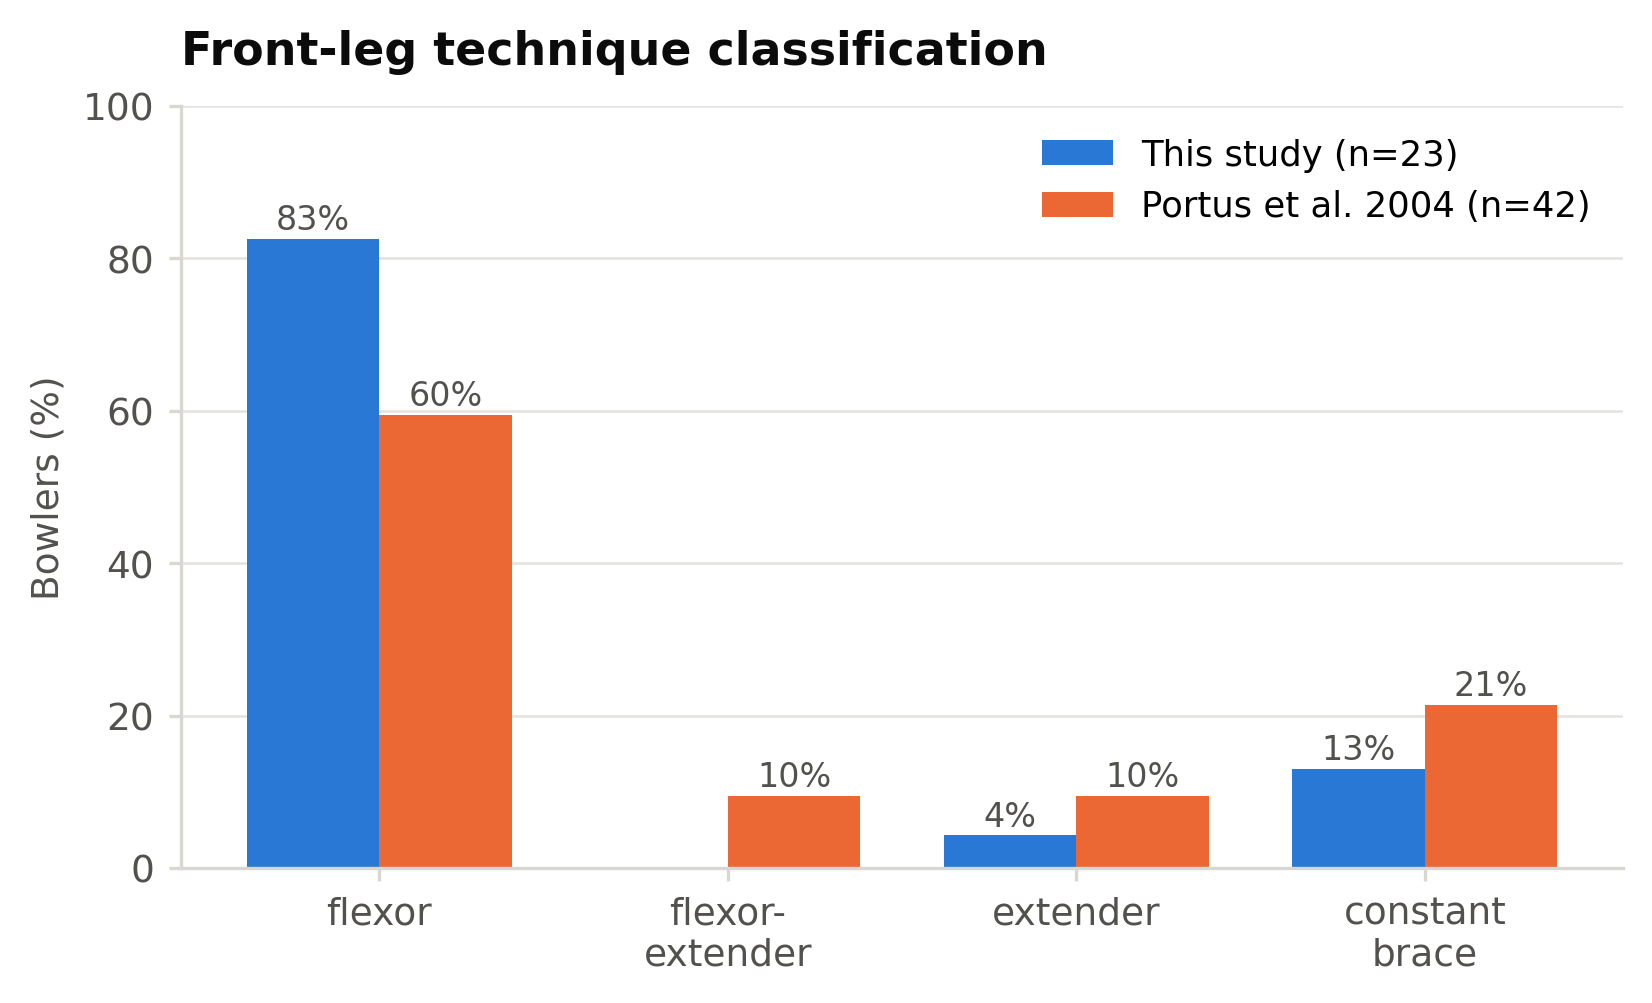
\includegraphics[width=0.78\textwidth]{fig8_technique.png}
  \caption{Front-leg technique against Portus et al.~\cite{portus2004}.}
  \label{fig:technique}
\end{figure}

Applying the classification of Portus et al.---a $10^\circ$ threshold on
flexion and on extension between FFC and release---19 of 23 bowlers (82.6\%)
are flexors against 59.5\% in the elite cohort. \textbf{One bowler in our
sample classifies as an extender and none as a flexor-extender}, 4.3\% combined
against 19\% in theirs, and three (13.0\%) are constant brace against 21.4\%.

\begin{table}[htbp]
  \centering
  \caption{Front-leg class per bowler. Consistency is the share of that bowler's own deliveries falling in their modal class.}
  \label{tab:techniqueperbowler}
  \begin{tabular}{lrrr}
    \toprule
    Bowler & Modal class & Deliveries & Consistency \\
    \midrule
    Anirudh & Flexor & 11/12 & 92\% \\
    Asish & Flexor & 15/15 & 100\% \\
    Charan & Constant brace & 5/9 & 56\% \\
    Hemanth & Extender & 12/13 & 92\% \\
    Jagan & Flexor & 12/12 & 100\% \\
    Jaswanth & Flexor & 4/8 & 50\% \\
    Junior1 & Flexor & 9/13 & 69\% \\
    Junior2 & Flexor & 11/11 & 100\% \\
    Junior3 & Flexor & 9/11 & 82\% \\
    Junior4 & Constant brace & 9/9 & 100\% \\
    Junior5 & Flexor & 4/4 & 100\% \\
    Jyothir & Flexor & 11/14 & 79\% \\
    Lohith & Flexor & 12/12 & 100\% \\
    Nithin & Flexor & 9/12 & 75\% \\
    Parthasaradhi & Flexor & 10/10 & 100\% \\
    Pradeep & Flexor & 9/10 & 90\% \\
    Prudhvi & Flexor & 13/13 & 100\% \\
    Ram & Flexor & 12/12 & 100\% \\
    SriMani & Constant brace & 10/12 & 83\% \\
    Srijay & Flexor & 11/11 & 100\% \\
    Suhail & Flexor & 13/13 & 100\% \\
    Umesh & Flexor & 14/14 & 100\% \\
    Vikhilesh & Flexor & 12/12 & 100\% \\
    \bottomrule
  \end{tabular}
\end{table}


Per-bowler classification also reports consistency---the share of a bowler's own
deliveries falling in their modal class. A bowler below roughly 70\% is not
reliably one class, and for them the group classification is a summary rather
than a description.

This corroborates the measurement result at two levels. At the group level, a
cohort in which knee extension is below elite for 22 of 23 bowlers produces
almost no extender classes, and the single extender is the single exception.
At the individual level, the four bowlers outside the flexor class---Charan,
SriMani and Junior4 as constant brace, Hemanth as extender---include all three
who depart from the group tendency on knee angle at release, as
Section~\ref{sec:universal} shows.

Hemanth's class should be read with care. His knee reads past straight at
release ($184^\circ$ on average), and in a single 2D view a nearly straight leg
is where landmark placement decides whether the knee sits a few pixels in
front of the hip--ankle line or behind it. Worthington observed the same
combination in his own cohort---the bowlers with the least flexion had the most
hyper-extended knees at release---so the reading is plausible, but it is the
measurement most exposed to pose error.

One definitional difference also leans towards the flexor class. Portus et
al.\ measure the front-knee phase from \emph{full} foot contact, the instant
the whole foot is down, to release; we measure from front foot contact, a few
frames earlier, because foot flat is not detected. Flexion counted from the
earlier instant reads larger (by a median of $5.6^\circ$ across our
deliveries), which can move a borderline bowler into the flexor class.
Beyond that, two readings remain open. Either club bowlers genuinely do not
brace and extend as professionals do, or our measurement systematically
compresses extension. We cannot distinguish them with the present data, and
prefer to say so.

\subsection{Limitations}
\label{sec:limits}

\paragraph{Ground truth is human annotation.} The reference marks were made by
one annotator, who is also an author. Published inter-annotator limits of
agreement on analogous gait events~\cite{gait2022} provide context, but an
independent second annotation of a random subset is required before these
figures should be treated as validated, and is the first item of future work.

\paragraph{Measurement accuracy is not validated.} We report that measurements
at detected instants are \emph{repeatable}, not that they are accurate in an
absolute sense. A multi-camera markerless system recorded $17.61 \pm
7.72^\circ$ RMSE on cricket bowling~\cite{abraham2025}; a single-camera 2D
pipeline should not be assumed to do better. The comparison with
Worthington is cross-study---different cohort, equipment and conventions---and
agreement indicates consistency, not accuracy.

\paragraph{The transverse plane is unrecoverable.} Shoulder counter-rotation,
which Portus et al.~\cite{portus2004} call the predominant technique factor in
lower-back injury, is a transverse-plane rotation of the shoulders between back
foot contact and the most side-on position just before front foot contact.
Colyer et al.~\cite{colyer2018} state the constraint precisely: a
two-dimensional analysis can recover only three of a segment's six degrees of
freedom, and reconstructing three-dimensional pose requires at least two camera
perspectives, which a single view cannot supply. The side-on / semi-open / front-on / mixed trunk
classification is therefore reported as \emph{not determinable from this data}.
We make no claim whatsoever about injury risk. A second camera placed behind
the bowler would supply the missing plane and is the clearest line of future
work.

\paragraph{Other limitations.} The trunk ratio $0.288$ is a population mean and
contributes roughly $\pm 2$--$3$ percentage points of individual error. Release
is detected at the wrist rather than the ball, biasing release height
approximately 10\,cm low; the per-bowler spread on that variable
(Section~\ref{sec:universal}) suggests it is also the least reliable of the
eight, and we draw no conclusion from it. Knee flexion is not compared with the
elite value because front foot flat is not detected; detecting it from the heel
and toe landmarks would restore the comparison but would first need hand marks
to validate against. The sample is 25 bowlers from one institute, one of
them excluded as not a trained bowler, with no injury outcomes.

\section{Conclusion}
\label{sec:conclusion}

Back foot contact, front foot contact and ball release can be located
automatically in fast-bowling video from a single uncalibrated side-on camera.
Ball release is found within 25\,ms on 98.5\% of deliveries and front foot
contact on 91.8\%, with no markers, no calibration and no laboratory. The
enabling idea is to train on phases and recover events from block edges; the
enabling engineering is normalisation to the bowler's own torso, which makes
camera geometry irrelevant.

Back foot contact remains the weak result at 59.0\%, and we have argued this is
a property of an event that rolls rather than arrives---supported both by the
ordering of our own three events and by published human annotation agreement on
analogous gait events. The bidirectional LSTM's performance there, 79.9\%
against 59.0\%, suggests long-range temporal context is the right remedy, and a
hybrid that uses sequence context for the diffuse event and local context for
the sharp one is the natural next step.

Finally, this work is as notable for what it declines to claim. The technique
factor most consistently linked to lower-back injury is a transverse-plane
quantity that one camera geometrically cannot recover. We
report it as unmeasurable rather than approximating it, because a confident
wrong number about a young athlete's injury risk is worse than an honest gap.

\refstepcounter{section}
\renewcommand{\refname}{\arabic{section}\quad References}
\addcontentsline{toc}{section}{References}
\begin{thebibliography}{99}

\bibitem{portus2004}
M.~Portus, B.~Mason, B.~Elliott, M.~Pfitzner, and R.~Done,
``Technique factors related to ball release speed and trunk injuries in high
performance cricket fast bowlers,''
\emph{Sports Biomechanics}, vol.~3, no.~2, pp.~263--284, 2004.

\bibitem{worthington2010}
P.~J.~Worthington,
\emph{A biomechanical analysis of fast bowling in cricket},
Ph.D. thesis, Loughborough University, 2010. Available:
https://hdl.handle.net/2134/6839.

\bibitem{colyer2018}
S.~L.~Colyer, M.~Evans, D.~P.~Cosker, and A.~I.~T.~Salo,
``A review of the evolution of vision-based motion analysis and the
integration of advanced computer vision methods towards developing a markerless
system,''
\emph{Sports Medicine --- Open}, vol.~4, no.~24, 2018.

\bibitem{winter1990}
D.~A.~Winter,
\emph{Biomechanics and Motor Control of Human Movement},
2nd ed., Wiley, 1990.

\bibitem{abraham2025}
A.~Abraham, S.~A.~Feros, and A.~S.~Fox,
``Exploring the accuracy of OpenCap for three-dimensional analysis of cricket
bowling,''
\emph{International Journal of Sports Science \& Coaching}, vol.~20, no.~6,
pp.~2571--2586, 2025, doi:10.1177/17479541251348081.

\bibitem{opencap2026}
X.~Zhang, D.~Mao, H.~Shang, L.~Ma, J.~Jia, J.~Yu, and M.~Zhang,
``Validations and applications of markerless motion capture using OpenCap: a
scoping review,''
\emph{Frontiers in Digital Health}, vol.~8, art.~1882536, 2026,
doi:10.3389/fdgth.2026.1882536.

\bibitem{marwah2025}
N.~Marwah,
``Cricket fast bowling optimization using machine learning pose estimation
modeling,'' preprint, Research Archive of Rising Scholars, 2025,
doi:10.58445/rars.2861.

\bibitem{illegal2026}
D.~Sutradhar, N.~Islam, S.~Mondal, T.~H.~Jamim, J.~M.~Shufol, and
S.~Shatabda,
``Deep learning based illegal bowling action detection,''
arXiv:2610.07223, 2026.

\bibitem{misbah2025}
Misbah-ur-Rehman, M.~R.~Abbas, M.~Rizwan, A.~Raza, and J.~Iqbal,
``A low-cost markerless motion-capture technique for early detection of
illegal cricket bowling action,''
\emph{Measurement Science and Technology}, vol.~36, art.~105418, 2025,
doi:10.1088/1361-6501/ae0ba2.

\bibitem{jayaweerage2024}
I.~Jayaweerage, K.~Rajamanthri, A.~Kothalawala, N.~Gunawardana, A.~Induranga,
P.~Weerakkody, K.~Maduwantha, and S.~Kumara,
``Motion capturing in cricket with bare minimum hardware and optimised
software: a comparison of MediaPipe and OpenPose,''
in \emph{Proc. 1st Int. Conf. on Software, Systems and Information Technology
(SSITCON)}, 2024.

\bibitem{pes2025}
H.~Xu, A.~Agrahari Baniya, S.~Wells, M.~R.~Bouadjenek, R.~Dazeley, and
S.~Aryal,
``Deep learning for sports video event detection: tasks, datasets, methods,
and challenges,''
arXiv:2505.03991, 2025.

\bibitem{gait2022}
J.~Wu, H.~Maurenbrecher, A.~Schaer, B.~Becsek, C.~Awai~Easthope,
G.~Chatzipirpiridis, O.~Ergeneman, S.~Pan\'e, and B.~J.~Nelson,
``Human gait-labeling uncertainty and a hybrid model for gait segmentation,''
\emph{Frontiers in Neuroscience}, vol.~16, art.~976594, 2022,
doi:10.3389/fnins.2022.976594.

\end{thebibliography}

\section{Contributions}

\noindent
\begin{tabular}{@{}ll>{\raggedright\arraybackslash}p{7.2cm}@{}}
  \toprule
  Roll number & Name & Contribution \\
  \midrule
  CS24B1031 & Alahari Tarak Ram & Organised both recording sessions;
    labelled the data, leading the frame-level annotation of 304
    deliveries. \\[3pt]
  CS24B1039 & Ponnangatti Bala Murugan & Designed the phase-reformulation
    approach; implemented the feature normalisation and temporal window
    stacking. \\[3pt]
  CS24B1046 & Vallipalli Lokesh Kumar & Implemented the event extraction and
    the kinematic measurement pipeline. \\[3pt]
  CS24B1069 & Bellala Parthasaradhi & Built the web application; conducted
    the literature review. \\
  \bottomrule
\end{tabular}

\medskip
\noindent All authors contributed to the analysis and to writing the report.

\end{document}
